\chapter{Refrigerantes}

\vspace{\fill}

\hrule

\vspace{.3cm}

{\large \lipsum[1]} 

\pagestyle{fancy}

\newpage


	\section{Refrigerantes}
	\Biblio{\cite[pág. 231 y 772 a 780]{Rajput2011termodinamica}}

	\begin{defs}
		Un \textbf{refrigerante} se define como cualquier sustancia que absorbe calor a través de su evaporación o condensación y lo pierde a través de su condensación solidificación en un sistema de refrigeración.
	\end{defs}

	Los refrigerantes logran el intercambio de calor siempre a partir de un medio mecánico, de modo que se cumpla la segunda ley de la termodinámica, la cual define que \emph{el calor, por sí mismo, no puede fluir de un cuerpo más frío a uno más caliente.}

	Los refrigerantes pueden clasificarse según la influencia sobre el medio a refrigerar, según su composición o según el entorno a enfriar. Tomando esta última clasificación se definen como:

	\begin{itemize}
		\item \textbf{Refrigerantes primarios.} Son aquellos refrigerantes que enfrían el medio a partir de la absorción del calor de forma latente. 
		\item \textbf{Refrigerantes secundarios.} Son aquellos refrigerantes que, se enfrían por medio de refrigerantes primarios, para luego absorber calor sensible del medio a refrigerar.
	\end{itemize}
	
	% \noindent Por otro lado, según la composición se definen como:

	% \begin{itemize}
	% 	\item \textbf{Compuestos de hidrocarburos}. Estos refrigerantes están conformados por enlaces químicos orgánicos, utilizando H y C en su totalidad, donde los enlaces entre átomos de H son simples. 
	% 	\item \textbf{Compuestos de halocarburos}. Estos refrigerantes derivan de hidrocarburos y están compuestos de carbono y elementos halógenos\footnote{Los halógenos son aquellos elementos de la tabla periódica del grupo 17: Flúor (F), cloro (Cl), bromo (Br) y yodo(I).}, principalmente Cl y F, aunque también puede presentarse Br o H (este último no forma parte de los halógenos). 
		
	% 	Dentro de los halocarburos se pueden encontrar algunas definiciones particulares:
	% 	\begin{itemize}
	% 		\item Clorofluorocarbonos (CFC): Refrigerantes compuestos en su totalidad por Cl, 
	% 		F y C.
	% 		\item hidroclorofluocarbonos (HCFC): Refrigerantes cuya composición solo tiene H, Cl, F y C.
	% 		\item Hidrofluorocarbonos (HFC): Refrigerantes cuya composición solo tiene H, F y C.
	% 		\item Hidrofluoolefinas (HFO): Refrigerantes cuya composición solo tiene H, F y olefinas (hidrocarburos insaturados que contienen al menos un doble enlace $C=C$).  
	% 	\end{itemize}

	% 	\item \textbf{Compuestos inorgánicos}. Estos refrigerantes están conformados por enlaces químicos no orgánicos. 
	% 	\item \textbf{Compuestos orgánicos insaturados}. Estos refrigerantes están conformados por enlaces químicos orgánicos, utilizando H y C, donde los enlaces entre átomos de H son dobles o triples. Además, puede presentarse en ellos Cl en algunos casos. 
	% \end{itemize}

	\section{Historia de los refrigerantes}
	\Biblio{\cite{calm2007next} \cite[pág. 29.5]{ashrae2017fundamentals}}

	La refrigeración parte de mucho tiempo atrás usando hielo almacenado, vaporización de agua u otros procesos de evaporación para evitar el calentamiento de objetos. 

	Numerosos investigadores en diferentes países estudiaron la física y química de los cambios de fase en el 1600s y 1700s; encontrando los fundamentos para lo que posteriormente se definiría como refrigeración artificial. Como primer actor de la refrigeración artificial, Oliver Evans propuso el uso de fluidos volátiles en un ciclo cerrado para congelar agua y formar hielo. El sistema descrito por Evans contemplaba un proceso de evaporación por vacío, enfriamiento del agua y posterior bombeo de vapor a un intercambiador de calor que permitía enfriar el gas para su reutilización. Y, aunque no se encuentran rastros de que Evans haya plasmado su idea en la realidad, probablemente estas hayan influenciado a Perkins y Trevithick. Este último propuso un sistema de refrigeración por ciclo de aire en 1828 pero, al igual que Evans, no construyó ninguno. Perkins, en cambio, si plasmó la idea y concretó la invención de la máquina de compresión de vapor los años 1830s, e introdujo el concepto de refrigerante así como lo conocemos hoy en día. Su patente de 1834 describe un ciclo de refrigeración utilizando un fluido volátil con el propósito de producir enfriamiento y congelamiento, y también la condensación de estos fluidos volátiles para permitir su reutilización sin desperdicio. Muchos expertos en refrigeración reconocen su contribución fundamental al identificar este método de compresión mecánica de vapor como el ciclo de Perkins.

	\begin{figure}[H]
		\centering
		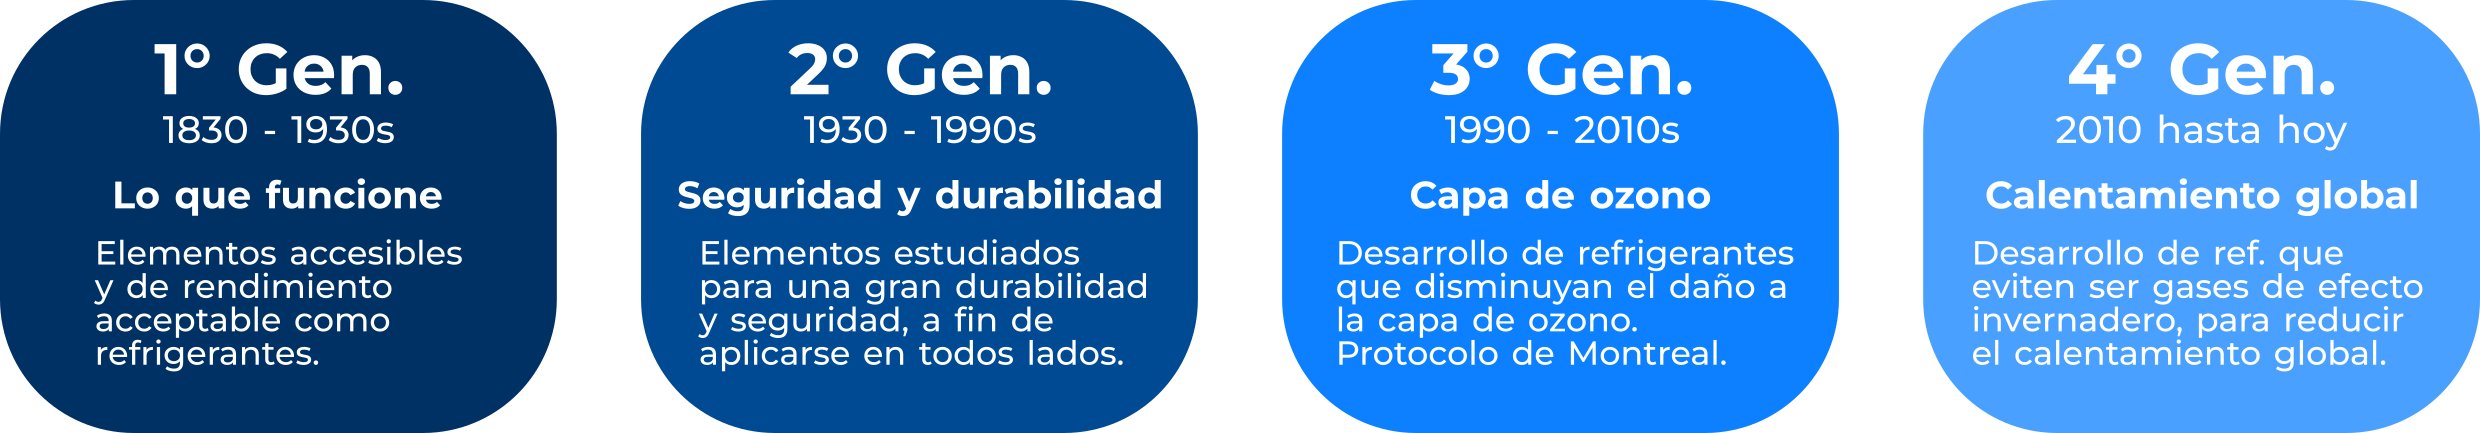
\includegraphics[width = 0.9\linewidth]{Figuras/U1/U1-Generaciones.png}
		\caption{Generaciones de refrigerantes.}\label{F1-Generaciones de refrigerantes}
	\end{figure}

	\subsection{Primera generación: \emph{lo que funcione}}
	
	Los refrigerantes más comunes de los primeros cien años de refrigeración eran solventes familiares y otros fluidos volátiles; la constitución de la primera generación de refrigerantes efectivamente incluía refrigerantes que funcionasen y estén disponibles. Casi todos estos refrigerantes eran tóxicos, inflamables o altamente reactivos con diferentes elementos constructivos. Los accidentes eran muy comunes. Para ponerlo en contexto, un gran número de compañías promovía el propano como un refrigerante seguro y sin olor, en contraparte al amoniaco. Además, este era publicitado como neutro químicamente, por lo que no reaccionaba con los elementos de las instalaciones, y que no era perjudicial ni desagradable, por lo que de ser necesario, los ingenieros podrían trabajar con propano en la atmósfera; ignorando completamente lo explosivo que podía resultar el mismo.

	La primera búsqueda sistemática documentada con el objetivo de mejorar el rendimiento de un sistema de refrigeración fue los años 1920's, enfocada principalmente a enfriadores. Willis H. Carrier, conocido por sus avances en la psicrometría y aire acondicionado, y R. W. Waterfill, investigaron un rango amplio de refrigerantes para el uso en compresores de desplazamiento positivo y turbocompresores radiales aplicados a enfriadores. Ellos concluyeron que el rendimiento del dióxido de carbono dependería del ciclo y la cantidad de subenfriamiento del líquido, pero que poseía el de rendimiento más bajo previsto entre los fluidos analizados. También notaron que la mezcla de amoniaco y agua  requeriría múltiples etapas de compresores centrífugos para obtener el rendimiento buscado, argumentando que el agua reducía la eficiencia del fluido. Rechazaron el dióxido de azufre por razones de seguridad y el tetracloruro de carbono por incompatibilidad con ciertos metales, especialmente en presencia de agua. Finalmente, seleccionaron el dicloruro de etileno para la primera máquina centrífuga, aunque esta selección requirió una búsqueda internacional para encontrar una fuente.

	\subsection{Segunda generación: \emph{Seguridad y durabilidad}}

	La segunda generación de refrigerantes estuvo impulsada por la pujante necesidad de aplicar la refrigeración a hogares. Con este enfoque, la industria de la refrigeración necesitaba un nuevo refrigerante si esperaban llegar a todos lados. Por tal motivo, Thomas Midgley Jr. y sus asociados Henne y McNary se enfocaron en encontrar un elemento que posea un punto de ebullición bajo. Además, redujeron su lista a elementos que sean estables, no sean tóxicos ni inflamables. Analizando publicaciones realizadas, la temperatura de ebullición del terafloruro de carbono llamó la atención sobre los fluoruros orgánicos, pero sospechaban correctamente que el valor real era mucho menor que el valor publicado. Al consultar la tabla periódica, Midgley descartó rápidamente aquellos elementos que producían una volatilidad insuficiente. Luego descartó aquellos que daban lugar a compuestos inestables y tóxicos, así como los gases inertes, basándose en sus bajos puntos de ebullición. Solo ocho elementos quedaron: carbono, nitrógeno, oxígeno, azufre, hidrógeno, cloro y bromo. Luego de tres días de empezar, en 1928, Midgley y sus compañeros hicieron observaciones críticas del comportamiento inflamable y tóxico de estos elementos. También notaron que todos los refrigerantes conocidos hasta el momento estaban compuestos por una combinación de siete de los ocho elementos seleccionados, todos menos el flúor. Su primera publicación luego de estos análisis mostró como el aditamento de cloro y flúor en refrigerantes generaba una variación en el punto de ebullición, la toxicidad y la inflamabilidad.

	La producción de refrigerante R12 comenzó en 1931 seguido del R11 en 1932. Los Clorofluorocarbonos como refrigerantes (CFCs) y los posteriores Hidroclorofluorocarbonos (HCFCs) dominaron la segunda generación de refrigerantes. El amoniaco continuó, así como lo hace hasta el momento, como el refrigerante más popular en sistemas industriales de gran magnitud, especialmente para el almacenamiento y procesado de comidas y bebidas.

	\subsection{Tercera generación: \emph{protección de la capa de ozono}}

	La vinculación de los CFCs con la reducción de la capa de ozono impulsó la tercera generación de refrigerantes. Esta generación tenía un enfoque claro, reducir el daño a la capa de ozono. Por tal motivo, se estableció una convención en Vienna con el objetivo de definir criterios que permitan limitar el daño, lo que consecuentemente resultó en el protocolo de Montreal, el cual forzó al abandono de sustancias que dañen o reduzcan la capa de ozono. Los químicos compuestos de flúor fueron el foco principal, con énfasis en los HCFCs como remplazo provisorio de los CFC y hidrofluorocarbonos (HFCs) como remplazo a largo plazo. Junto a esto, este protocolo volvió a traer un gran interés en los refrigerantes naturales, principalmente amoniaco, dióxido de carbono, hidrocarburos y agua. Existieron muchos programas públicos y privados para obtener refrigerantes sin flúor o con el flúor junto a éteres (HFE: hidrofluoruroeter), pero no se obtuvieron resultados prometedores.
	
	Recién en 1989 los fabricantes comercializaron los primeros refrigerantes prometedores. Durante los años consecuentes fueron presentando alternativas a los refrigerantes que dañaban la capa de ozono.

	Con el fin de lograr un cambio progresivo, en el protocolo de Montreal se establecieron dos tipos de países, desarrollados y no desarrollados. Los desarrollados tuvieron como objetivo dejar de utilizar refrigerantes CFCs en equipamientos nuevos para el año 1996, mientras que los subdesarrollados tenían un lapso mayor, permitiendo su uso hasta 2010. Sin embargo, no se limitó el uso de refrigerantes en sistemas preexistentes. 

	Así como con los CFCs, sobre los HCFCs se estableció un límite temporal a cumplir, ya que su aplicación en nuevos sistemas era provisoria. Lo establecido en el protocolo de Montreal fue reducir progresivamente el uso de HCFCs de modo que en 2004 existiesen un 65\% del total de sistemas de refrigeración en HCFCs, en 2010 un 25\%, en 2015 un 10\%, en 2020 un 0.5\%, y hasta extinguirse por completo en 2030 en los países desarrollados; en países subdesarrollados los límites temporales fueron en 2015 un 90\%, 2020 un 65\%, en 2025 un 32.5\%, en 2030 un 2.5\% seguido de una extinción completa en 2040.

	\subsection{Cuarta generación: \emph{calentamiento global}}

	La cuarta generación, desarrollada en la actualidad, posee un vínculo estrecho con el calentamiento global. La temperatura global promedio es determinada por un balance entra la energía del sol calentando la tierra y la energía radiada por la tierra al espacio. En este análisis los gases de efecto invernadero, como el dióxido de carbono, vapor de agua y algunos refrigerantes, atrapan el calor sobre la superficie aumentando la temperatura a valores mayores de los esperados.

	Realizados estudios que relacionan la actividad humana con el efecto invernadero, es notable que la existencia de gases de efecto invernadero aumentó intensamente con el desarrollo tecnológico de la humanidad. Y, aunque el mayor gas de efecto invernadero es el dióxido de carbono, el metano, óxido nitroso, CFCs, HCFCs, HFC, éteres y olefinas de hidrógeno y flúor, SF6 son también gases de efecto invernadero (entre otros).
	 
	Por tal motivo, la cuarta generación de refrigerantes tiene como objetivo reducir el calor almacenado por las partículas de refrigerante filtradas a la atmósfera. Para lograr esto, se deberá considerar como criterio principal la duración los compuestos en la atmósfera y el calor que estos pueden retener allí.

	\newpage 
	\section{Composición de los refrigerantes}
	\Biblio{\cite[pág. 388 a 390]{DossatPDRefrigeracion} \cite[pág. 772 a 773]{Rajput2011termodinamica}  \\ \cite[pág. 29.2 a 29.5]{ashrae2017fundamentals} \cite[pág. 890 a 905]{Whitten2016quimica}}

	\subsection{Refrigerantes de hidrocarburos}

	La mayoría de los refrigerantes de este grupo son compuestos orgánicos. Varios hidrocarburos se emplean con éxito en  instalaciones comerciales e industriales. Casi todos estos poseen propiedades térmicas satisfactorias, pero son altamente inflamables. Algunos de los refrigerantes de hidrocarburos se presentan en la figura \ref{F1-Hidrocarburos}. 

	\begin{figure}[H]
		\centering
		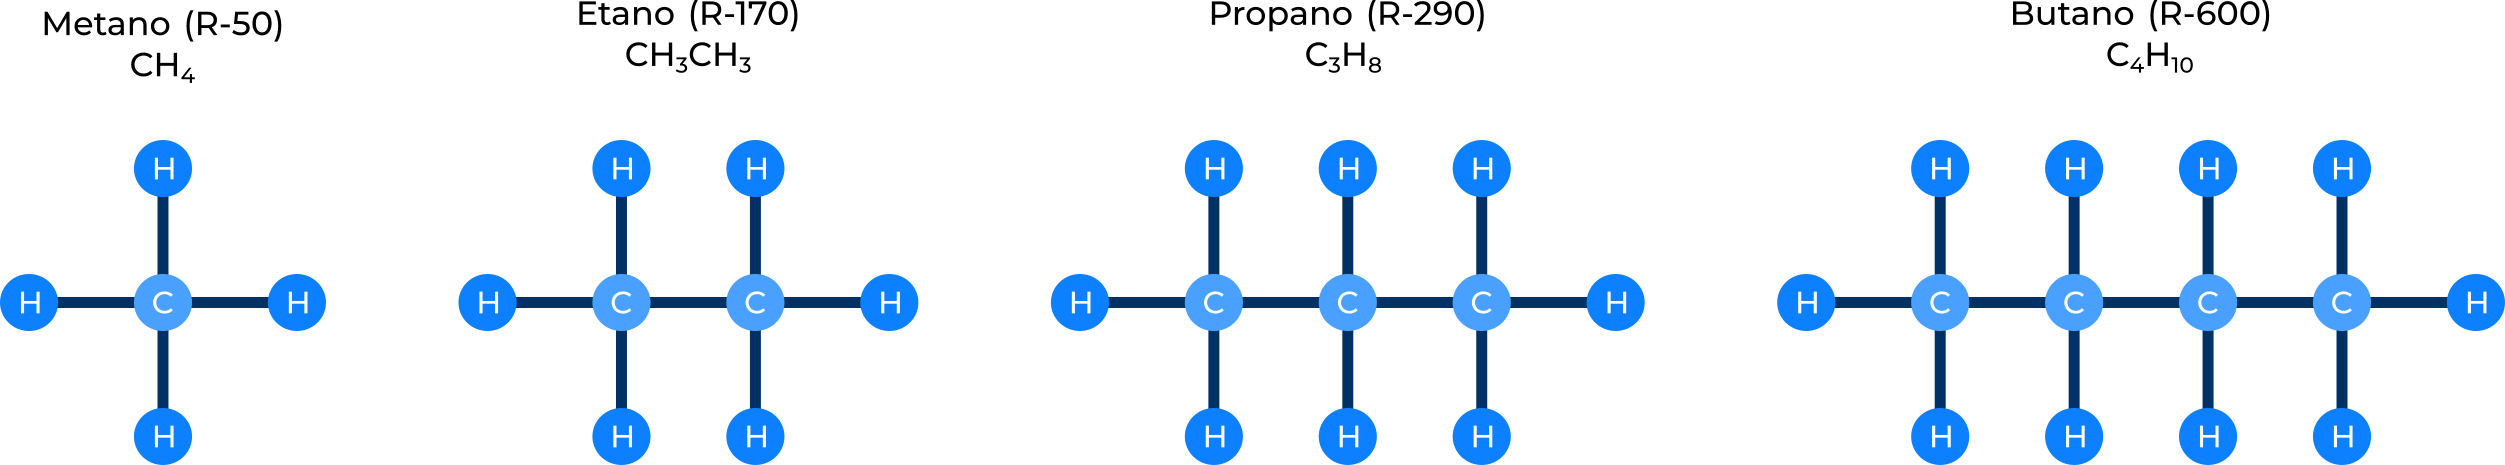
\includegraphics[width = \linewidth]{Figuras/U1/U1-CompuestosHidrocarburos.png}
		\caption{Moléculas de hidrocarburos.}\label{F1-Hidrocarburos}
	\end{figure}

	La nomenclatura del metano, el etano y el propano siguen una regla posteriormente desarrollada explicando los halocarburos, mas el butano posee una nomenclatura elegida arbitrariamente.

	\subsection{Refrigerantes de halocarburos}

	Los refrigerantes de segunda generación tuvieron como objetivo ser seguros y tener buenas propiedades térmicas, como se indicó anteriormente estos estaban conformados principalmente por H, F, Cl, C, N, O, S y Br. A este grupo de refrigerantes se lo denomina refrigerantes halogenados, ya que derivan de hidrocarburos y son modificados por elementos halógenos (del grupo XVII de la tabla periódica).
	
	Para obtenerlos se modificaron moléculas de etano y de metano, introduciendo principalmente cloro y flúor en sus enlaces simples.

	\begin{figure}[H]
		\centering
		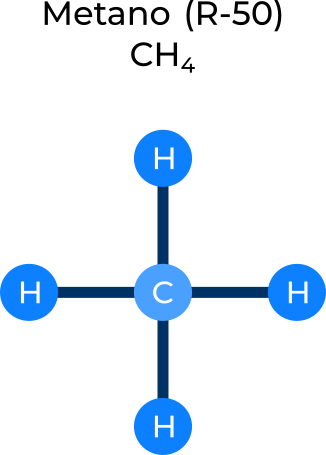
\includegraphics[width = 0.19\linewidth]{Figuras/U1/U1-Metano.png}
		\caption{Molécula de metano.}\label{F1-Molécula de metano}
	\end{figure}

	Tomando la molécula de metano (fig. \ref{F1-Molécula de metano}) es posible obtener los refrigerantes de las series R40, R30, R20 y R10 remplazando las moléculas de hidrógeno por cloro y luego por flúor. Para comprender mejor la obtención y la nomenclatura, la figura \ref{F1-Desarrollo de refrigerantes derivados del metano} ofrece un desarrollo de cómo se llega a cada refrigerante derivado del metano. Para ejemplificarlo se analiza el R22. Para construir R22 se debe constituir inicialmente cloroformo (refrigerante R20), el cual se obtiene remplazando tres átomos de hidrógeno por tres de cloro, dejando dos átomos iniciales de la molécula (el carbono y un hidrógeno). Luego de haber conformado el R22, sobre los cloros presentes, se remplazan dos átomos de cloro por átomos de flúor, obteniendo así el R22. Para una mejor compresión es posible dar otro ejemplo, en este caso la conformación de R12. En este caso se remplazan cuatro átomos de hidrógeno por átomos de cloro, dejando un único átomo de los originales, el carbono; obteniendo así Carbonotetracloruro (refrigerante R10). Una vez echo esto, se remplazan dos átomos de cloro por dos átomos de flúor, llegando así al R12.

	\begin{figure}[H]
		\centering
		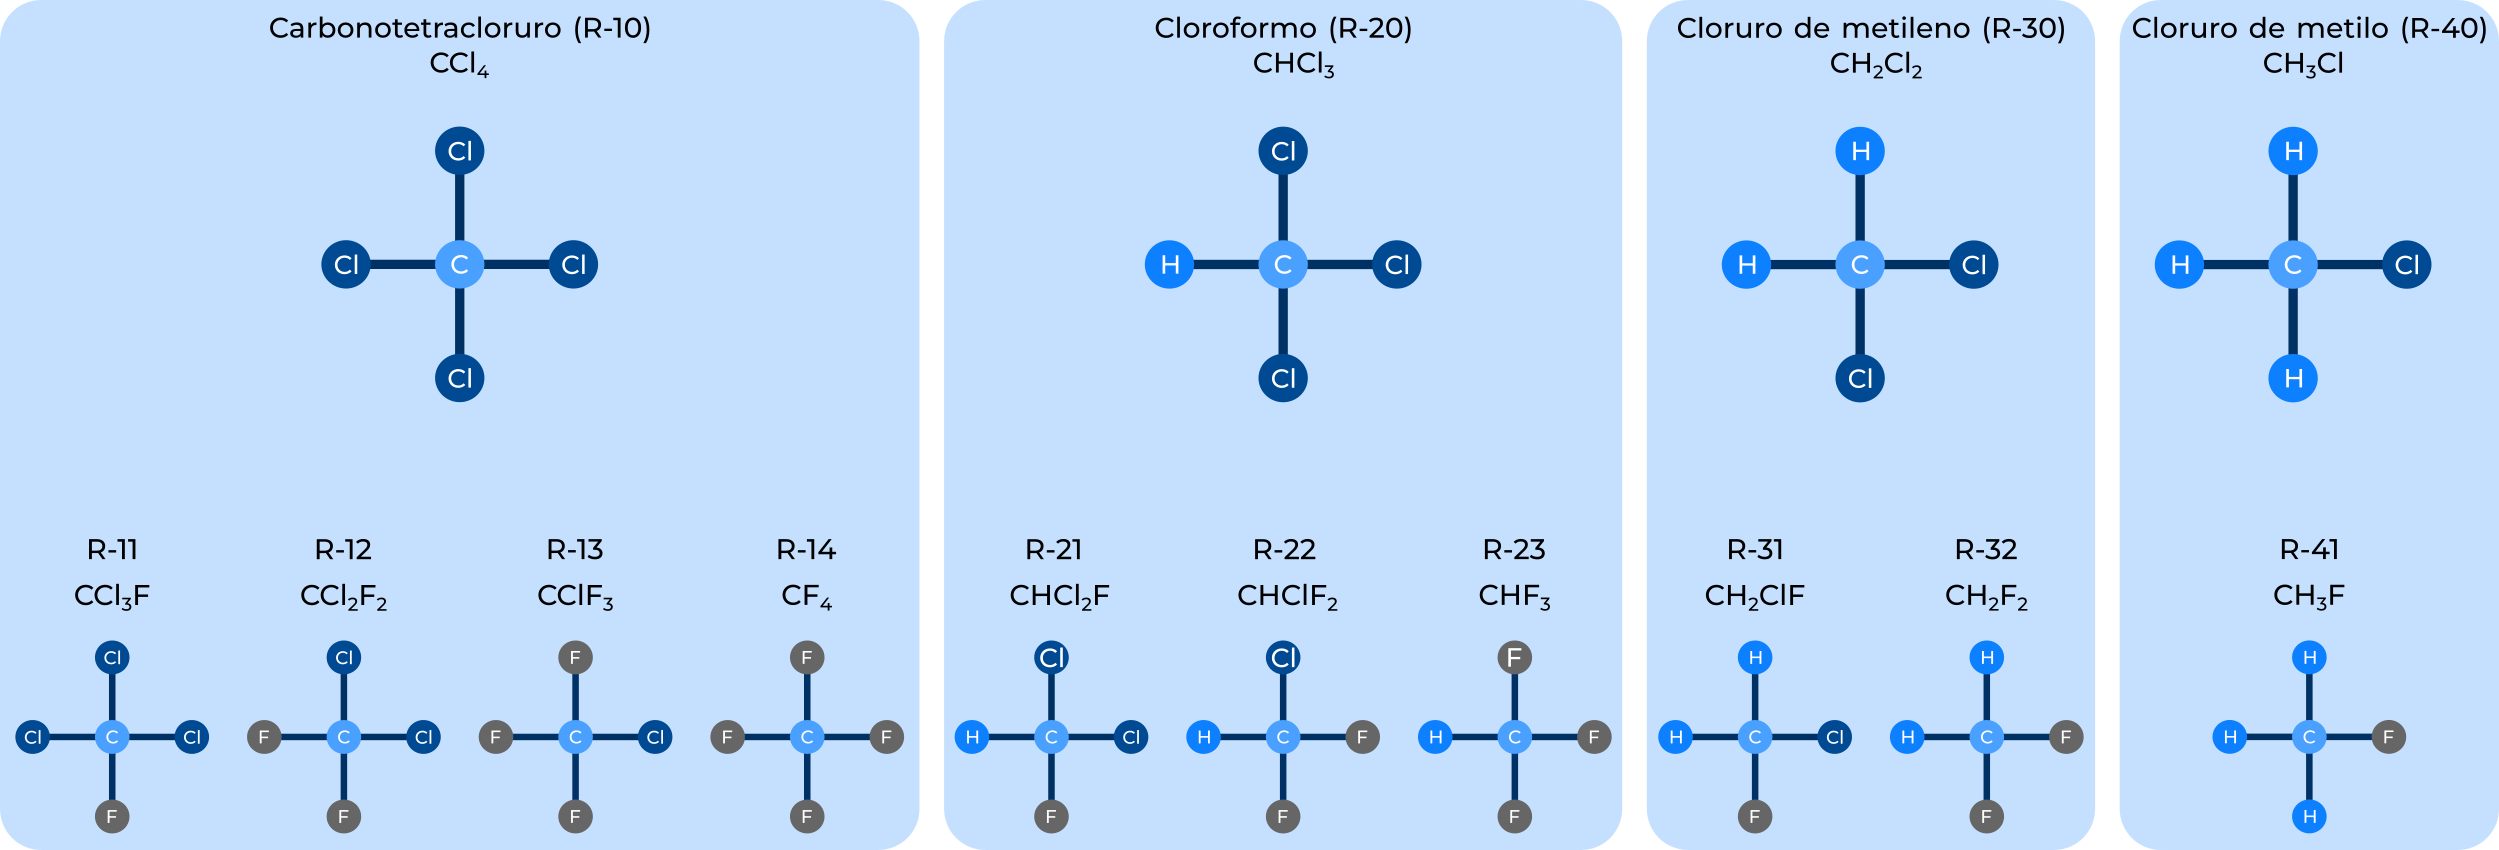
\includegraphics[width = \linewidth]{Figuras/U1/U1-DesarrolloMetano.png}
		\caption{Desarrollo de refrigerantes derivados del metano.}\label{F1-Desarrollo de refrigerantes derivados del metano}
	\end{figure}

	Si se prestó atención en los ejemplos desarrollados anteriormente, es posible deducir el significado de la nomenclatura de los refrigerantes derivados del metano. En ellos las dos cifras combinadas luego de la letra R indican:

	\begin{itemize}
		\item Primera cifra: Cuantos átomos de la molécula original no fueron reemplazados por cloro, considerando al carbono como irreemplazable.
		\item Segunda cifra: Cuantos átomos de cloro presentes fueron reemplazados por átomos de flúor.
	\end{itemize}

	\begin{figure}[H]
		\centering
		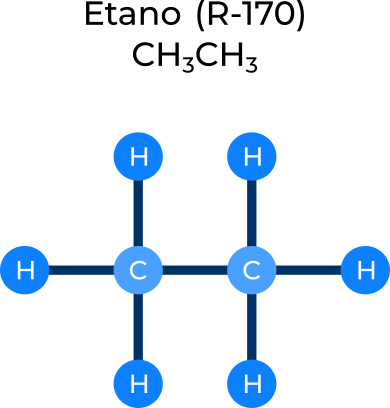
\includegraphics[width = 0.22\linewidth]{Figuras/U1/U1-Etano.png}
		\caption{Molécula de etano.}\label{F1-Molécula de etano}
	\end{figure}

	Con los refrigerantes derivados del etano sucede algo similar, para comprender esto primero se visualiza la molécula de etano (fig. \ref{F1-Molécula de etano}). A partir de esta molécula es posible obtener la serie de refrigerantes R110 a R160 remplazando los átomos de hidrógeno por átomos de cloro, y luego estos por átomos de flúor. Para comprender mejor la nomenclatura se presenta la figura \ref{F1-Desarrollo de refrigerantes derivados del etano}, donde se muestra la composición de las moléculas de algunos refrigerantes derivados del etano. Con fines didácticos, se desarrolla como ejemplo la obtención de R134, para este primero hay que obtener R130, por lo que se toma la molécula de etano y se remplazan cuatro hidrógenos por cuatro cloros, dejando cuatro átomos iniciales de la molécula (dos carbonos y dos hidrógenos). Luego de obtenido el R130, se remplazan cuatro átomos de cloro por cuatro átomos de flúor, obteniendo así el R134. 

	\begin{figure}[H]
		\centering
		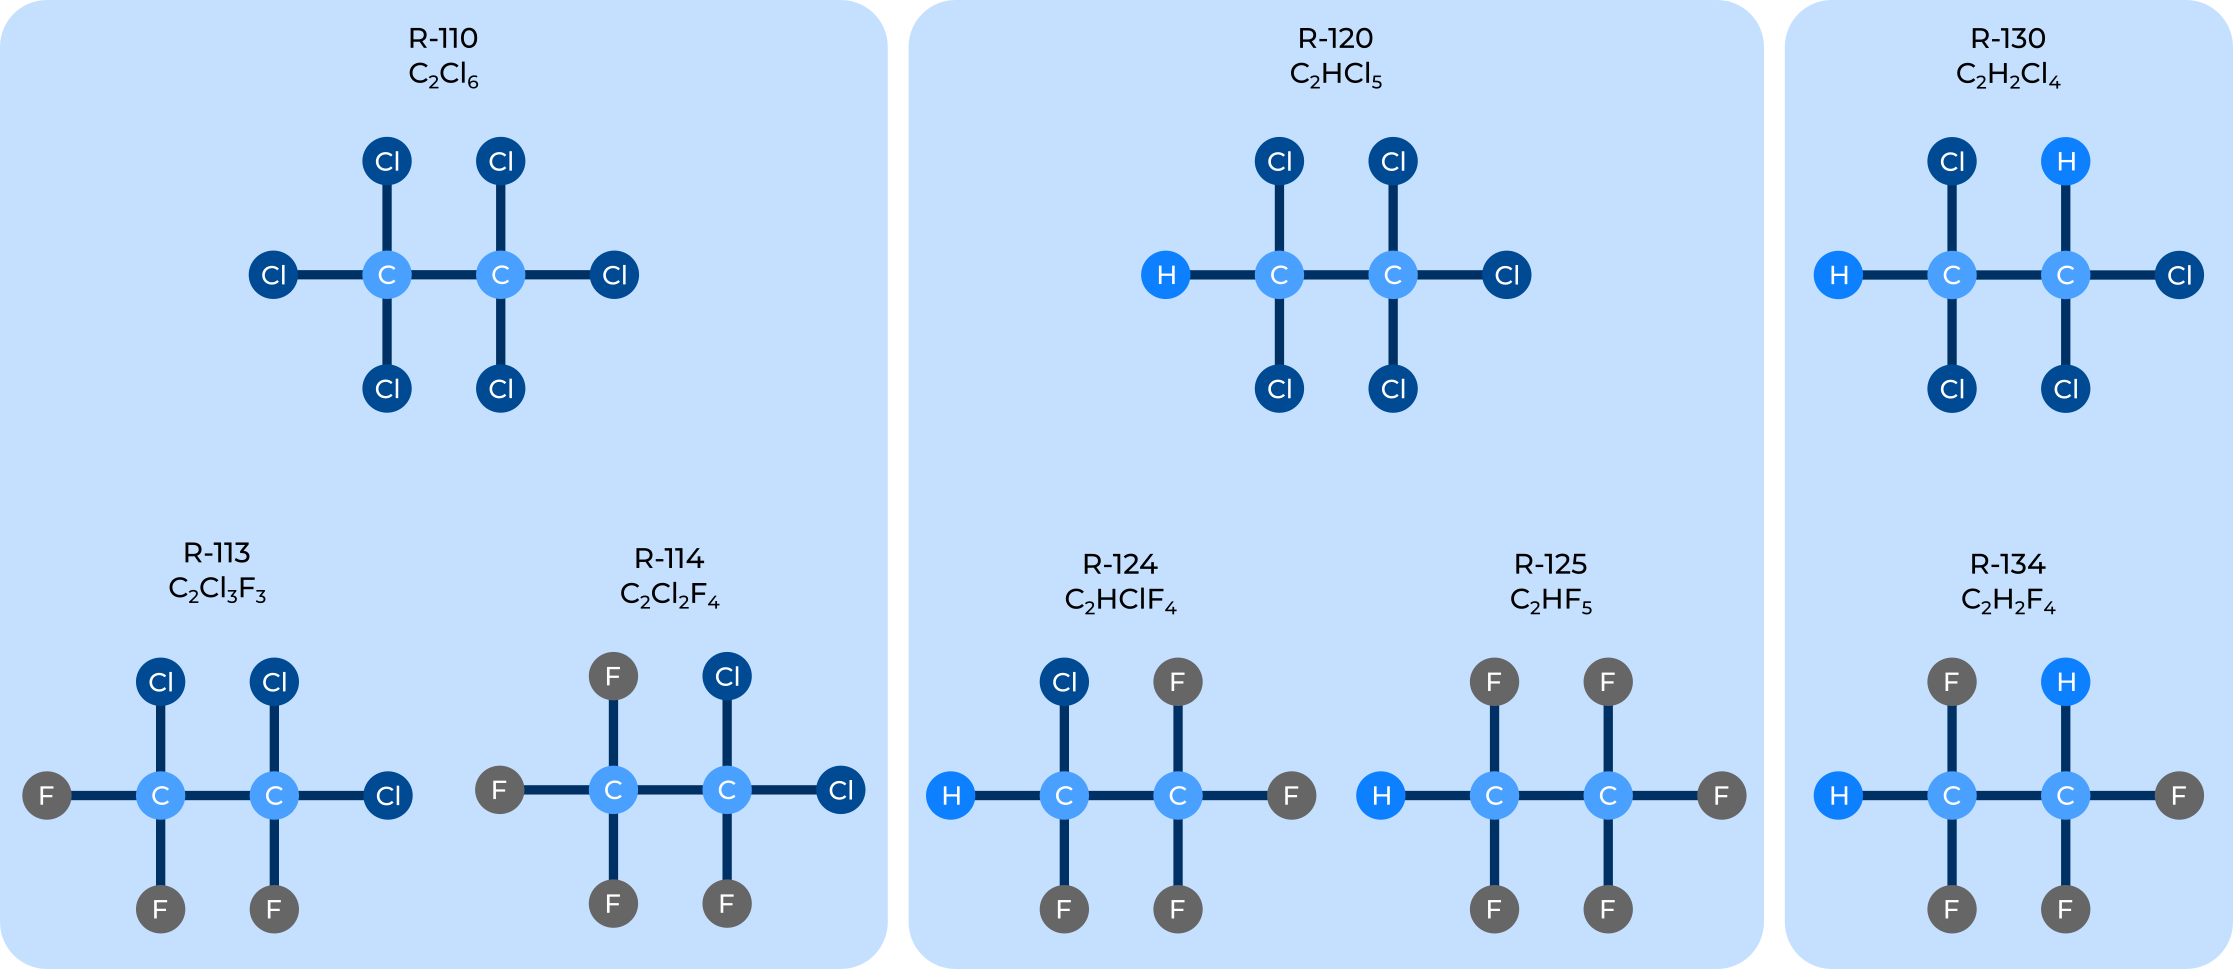
\includegraphics[width = \linewidth]{Figuras/U1/U1-DesarrolloEtano.png}
		\caption{Desarrollo de refrigerantes derivados del etano.}\label{F1-Desarrollo de refrigerantes derivados del etano}
	\end{figure}

	Aquí, a diferencia de los refrigerantes derivados del metano, la nomenclatura no es tan evidente, pero una vez comprendida resulta clara. Para comprender esta se analiza que, luego de la R:

	\begin{itemize}
		\item Primera cifra: indica la existencia de un átomo de carbono adicional dentro de la molécula.
		\item Segunda cifra: indica cuántos átomos de la molécula original, sin contar el carbono adicional no fueron remplazados por el cloro, considerando a los carbonos irreemplazables. 
		\item Tercera cifra: indica cuantos átomos de cloro presentes fueron reemplazados por átomos de flúor.
	\end{itemize}

	\subsection{Refrigerantes inorgánicos - R700s}

	Los compuestos inorgánicos eran aquellos refrigerantes que se encontraban con frecuencia o se podían conformar fácilmente en los comienzos de la refrigeración, por lo que definieron la primer generación de refrigerantes. Estos fueron principalmente amoniaco, agua, aire, dióxido de carbono y dióxido de azufre.

	\begin{figure}[H]
		\centering
		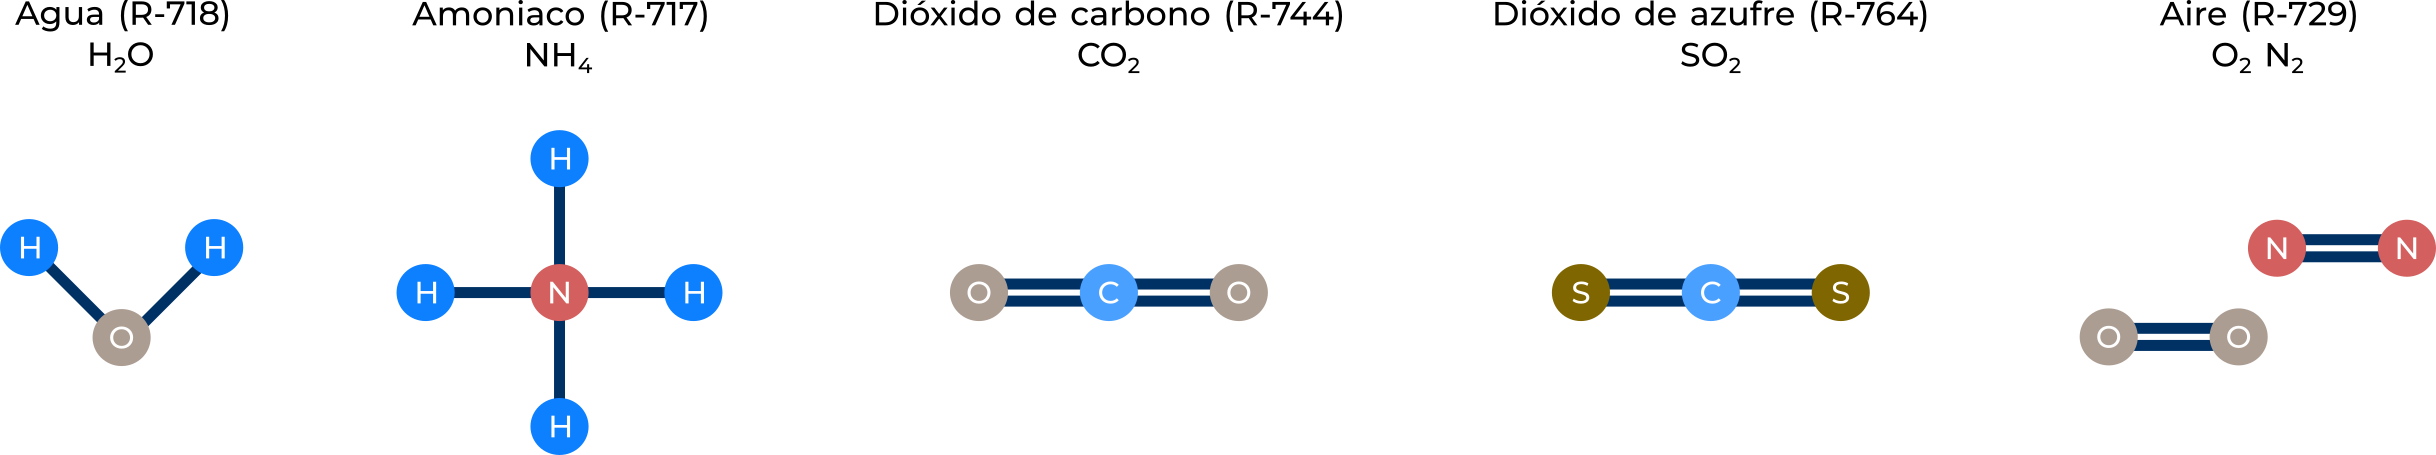
\includegraphics[width = \linewidth]{Figuras/U1/U1-CompuestosInorganicos.png}
		\caption{Moléculas de inorganicos.}\label{F1-Inorganicos}
	\end{figure}
	
	Estos refrigerantes están identificados por tres cifras de forma arbitraria, donde su primera cifra siempre será un 7.

	\newpage

	\subsection{Refrigerantes azeótropos - R500}

	Los refrigerantes que pertenecen a este grupo consisten en mezclas de sustancia diferentes. Estas sustancias no se pueden separar en sus componentes mediante destilaciones. Poseen propiedades térmicas fijas y no experimentan separación con cambios en temperatura y presión. Un azeótropo se comporta como una sustancia simple. A continuación se muestra un par de refrigerantes azeótropos en la tabla \ref{T1-Algunos refrigerantes azeótropos.}.

	\begin{table}[H]
		\centering
		\small
		\caption{Algunos refrigerantes azeótropos.}\label{T1-Algunos refrigerantes azeótropos.}
		\begin{tabular}{C{0.2\linewidth} C{0.2\linewidth} C{0.2\linewidth} C{0.2\linewidth}}
			Refrigerante & Composición & Porcentajes & Tolerancias \\
			\hline
			R500 & R12 + R152a & 73\% + 26.2\% & - \\
			R502 & R22 + R115 & 48.8\% + 51.2\% & - \\
			R503 & R23 + R13 & 40.1\% + 59.9\% & - \\
			R507A & R125 + R143a & 50\% + 50\% & - \\
			R508A & R23 + R116 & 39\% + 61\% & - \\
			R508B & R23 + R116 & 46\% + 54\% & - \\
			\hline
			\multicolumn{4}{M{0.85\linewidth}}{\footnotesize Los refrigerantes acompañados de la letra \cmll{a} representan compuestos derivados de isómero.}
		\end{tabular}
	\end{table}

	La nomenclatura de los refrigerantes azeótropos, así como los inorgánicos, se definieron de forma secuencial a partir del número 500. Donde, en caso de presentarse dos o más combinaciones de los mismos refrigerantes,  pero con diferentes variantes de porcentaje, el código es acompañado de una letra mayúscula a la derecha, indicando el tipo de variante que es.

	\subsection{Refrigerantes zeótropos - R400}

	Los refrigerantes zeótropos son aquellos que consisten en mezclas de sustancias diferentes y se comportan como sustancias diferentes frente a los cambios de temperatura y presión, principalmente cuando se presentan como vapor. A continuación se muestra un par de refrigerantes zeótropos en la tabla \ref{T1-Algunos refrigerantes zeótropos.}.

	\begin{table}[H]
		\centering
		\small
		\caption{Algunos refrigerantes zeótropos.}\label{T1-Algunos refrigerantes zeótropos.}
		\begin{tabular}{C{0.18\linewidth} C{0.25\linewidth} C{0.22\linewidth} C{0.2\linewidth}}
			Refrigerante & Composición & Porcentajes & Tolerancias \\
			\hline
			R404A & R125 + R143a + R134a & 44\% + 52\% + 4\% & ($\pm 2$, $\pm 1$, $\pm 2$) \\
			R407A & R32 + R125 + R134a & 20\% + 40\% + 40\% & ($\pm 2$, $\pm 2$, $\pm 2$) \\
			R407C & R32 + R125 + R134a & 23\% + 25\% + 52\% & ($\pm 2$, $\pm 2$, $\pm 2$) \\
			R410A & R32 + R125 & 50\% + 50\% & ($+0.5 \, -1.5$, $+1.5 \, -0.5$) \\
			\hline
			\multicolumn{4}{M{0.87\linewidth}}{\footnotesize Los refrigerantes acompañados de la letra \cmll{a} representan compuestos derivados de isómero.}
		\end{tabular}
	\end{table}

	La nomenclatura de los refrigerantes zeotrópicos también están definidas de forma secuencial a partir del número 400, donde también se cumple la regla de que los refrigerantes que posean la misma composición pero con diferentes porcentajes se diferencian por una letra mayúscula luego del código alfanumérico.

	\subsection{Refrigerantes orgánicos insaturados}

	Para analizar los refrigerantes orgánicos insaturados, primero se define hidrocarburos saturados e insaturados. Los hidrocarburos saturados son aquellos que cada átomo de carbono está unido a otros cuatro átomos, comúnmente denominado alcanos. Por otro lado, existen dos tipos de hidrocarburos insaturados: alquenos, que poseen un doble enlace entre carbonos por molécula; y alquinos, que poseen uno o más enlaces triples entre carbonos por molécula.	El término saturado proviene de los primeros estudios en los cuales los químicos trataron de agregar hidrógeno a varias sustancias orgánicas. Aquellas a las que no podía agregarse más hidrógeno recibieron el nombre de saturadas, por analogía de las soluciones saturadas.

	\begin{figure}[H]
		\centering
		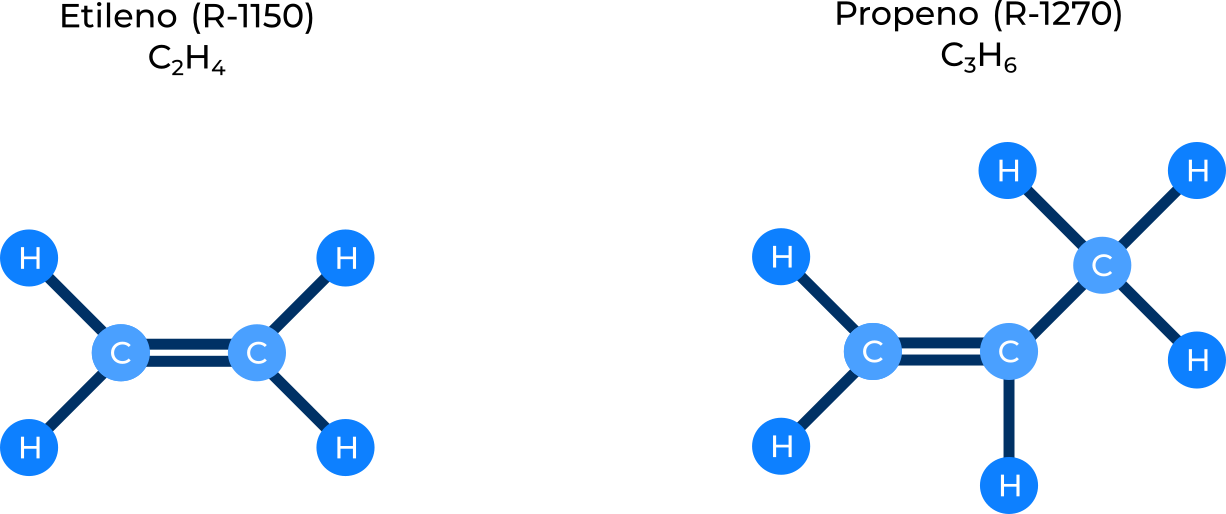
\includegraphics[width = 0.6\linewidth]{Figuras/U1/U1-OrgInsat.png}
		\caption{Propeno y etileno - Orgánicos insaturados.}\label{F1-Organicos Insaturados}
	\end{figure}

	Dicho esto, en la figura \ref{F1-Organicos Insaturados} se presentan moléculas de propeno y etileno, las cuales son bases para algunos refrigerantes orgánicos insaturados. A partir de ellos, se constituyen los refrigerantes de series R1100 y R1200, donde su nomenclatura y composición es similar a aquella detallada en los refrigerantes de halocarburos. Para dar un ejemplo práctico de obtención, se analiza como se compone el R1234. Este refrigerante comienza siendo una molécula de propeno sobre la cual se remplazan cuatro átomos de hidrógeno por átomos de cloro, dejando de la molécula inicial, dos átomos de hidrógeno, y tres de carbono donde dos están enlazados de manera doble. Una vez realizado esto, se remplazan cuatro átomos de cloro por átomos de flúor, logrando así la estructura requerida para un R1234.

	\begin{figure}[H]
		\centering
		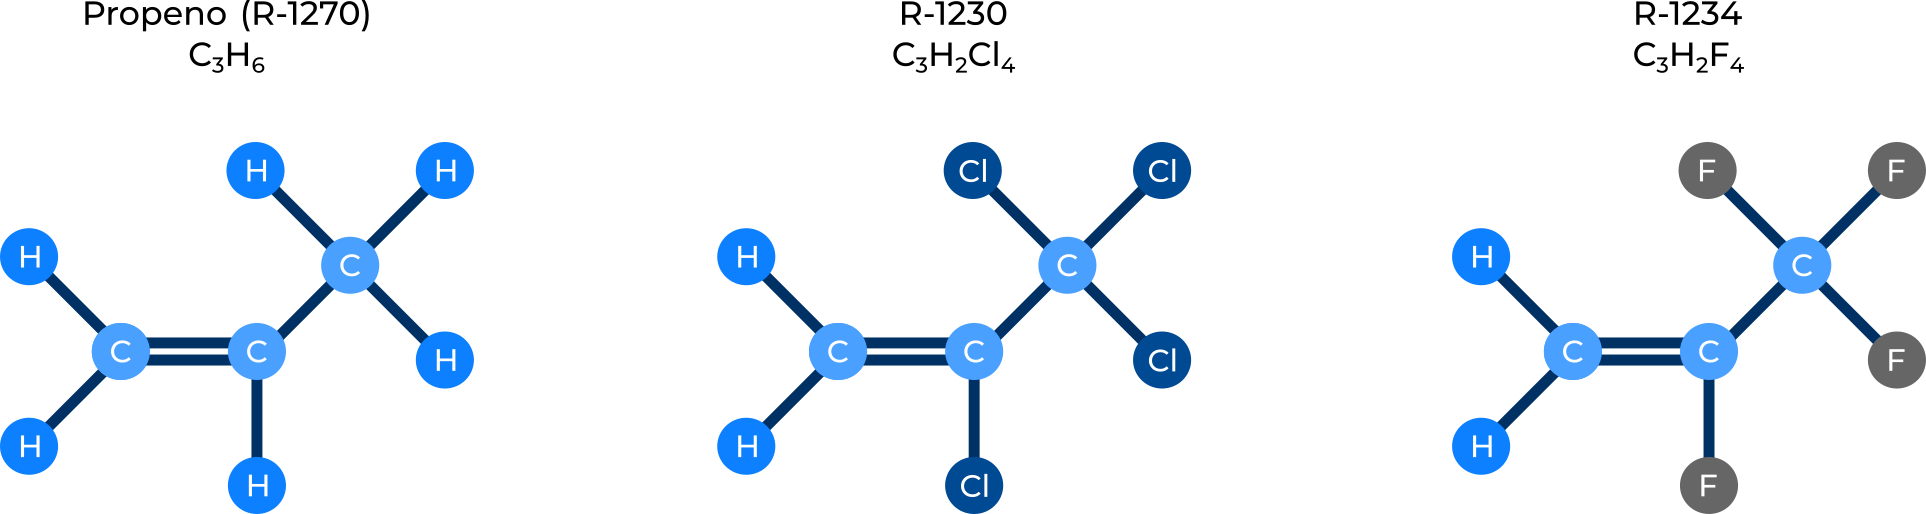
\includegraphics[width = 0.9\linewidth]{Figuras/U1/U1-PropenoA1234.png}
		\caption{Desarrollo de propeno a R1234.}\label{F1-Propeno a R1234}
	\end{figure}

	Al igual que los refrigerantes derivados de hidrocarburos saturados, la nomenclatura de los refrigerantes orgánicos insaturados define la composición de la siguiente manera:

	\begin{itemize}
		\item Primera cifra: indica la presencia de un enlace doble en la molécula, definiendo que es una molécula orgánica insaturada.
		\item Segunda cifra: indica la cantidad de átomos de carbono que posee la molécula, restando uno. 
		\item Tercera cifra: indica la cantidad de átomos originales no fueron reemplazados por cloro y permanecen en la molécula. Considerando a todos los átomos de carbono como un único elemento original. 
		\item Cuarta cifra: indica cuantos átomos de cloro fueron reemplazados por flúor.
	\end{itemize}

	\section{Características de un refrigerante ideal}
	\Biblio{\cite[pág. 19]{mott2015fluidos} \cite[pág. 774 a 789]{Rajput2011termodinamica} \cite[pág. 33, 36, 68, 69, 385 a 395]{DossatPDRefrigeracion} \\ \cite[pág. 57, 158, 167, 168 y 177]{miller2006refrigeration}  \cite[pág. 800 y 802]{askeland2017materiales} \cite[pág. 2.15]{ashrae2017fundamentals} }

	Las propiedades deseables de un refrigerante ideal son aquellas que permiten absorber mayor cantidad de calor realizando el menor trabajo posible, y trabajar en rangos amplios de temperatura. A estas características es posible separarlas en cuatro grupos: 

	\begin{multicols}{2}
	\begin{itemize}
		\item Propiedades termodinámicas.
		\item Propiedades químicas.
		\item Propiedades físicas.
		\item Propiedades varias.
	\end{itemize}

	\end{multicols}

	\subsection{Propiedades termodinámicas}
	
	\paragraph{Punto de congelación} El punto de congelación de una sustancia es aquella temperatura en la que una sustancia, a una presión determinada, cambia de estado líquido a sólido. 

	Los refrigerantes utilizados que sean aplicados en ciclos de condensación-evaporación deberán siempre tener un punto de congelación más bajo que la temperatura mínima del sistema a las presiones de trabajo.

	\paragraph{Presión del condensador} La presión del condensador es el valor de presión a la cual el condensador realiza el intercambio de calor con el medio.

	Este valor depende exclusivamente de la presión que se presente en el evaporador y el aumento de presión realizado por el compresor, ya que el condensador se encuentra a la salida de éste. Considerando esto, obtener una presión de condensador baja permite utilizar equipos que requieran menor resistencia y sean más económicos.
	
	\paragraph{Presión del evaporador} La presión del evaporador es el valor de presión a la cual el evaporador realiza el intercambio de calor con el medio.

	En los sistemas de refrigeración la presión de evaporación debe estar lo más cerca de la presión atmosférica como sea posible y ser positiva. Una presión positiva se requiere a fin de eliminar la posibilidad de entrada de aire y humedad en el sistema. Se debe tener en cuenta que las presiones bajas presentan grandes volúmenes de aspiración para el compresor. Por tal motivo, debe ser una variable a tener en cuenta.

	%	\paragraph{Presiones del condensador y del evaporador} La presión de evaporación debe estar tan cerca de la atmosférica como sea posible. Si es demasiado baja, resultaría en un gran volumen de vapor de aspiración. SI es demasiado alta, las presiones globales altas, incluyendo la presión del condensador, resultarían en la necesidad de equipo más resistente y en consecuencia en un costo mayor. 

	%	Una presión positiva se requiere a fin de eliminar la posibilidad de entrada de aire y la humedad en el sistema. Por lo tanto, el punto de ebullición normal de un refrigerante deberá ser menor que la temperatura del refrigerante.

	\paragraph{Temperatura crítica} La temperatura crítica es el último valor de temperatura en que el vapor puede condensarse completamente mediante el aumento de presión. A partir de este valor, sin importar la presión que se presente, el fluido se presenta en estado gaseoso sin condensarse completamente. A medida que la temperatura se acerca al valor crítico, el fluido absorbe menor cantidad de calor en el cambio de estado.

	La temperatura crítica de un refrigerante debe encontrarse por encima de la temperatura de condensación, idealmente presentando una gran diferencia. Esto permite mayor disipación de calor del refrigerante al medio, logrando un mejor rendimiento térmico.
	
	\newpage

	\paragraph{Presión crítica} La presión crítica es el valor de presión mínimo que requiere el refrigerante en el umbral de temperatura crítica para condensarse. 

	En los sistemas de refrigeración, una presión crítica baja representa la posibilidad de ciclos a bajas presiones, debido a que, mientras más baja la presión crítica, más bajas pueden ser las presiones de condensación y evaporación. 
	
	\paragraph{Temperatura de saturación} Es la temperatura a la cual un fluido pasa de fase líquida a fase de vapor, o a la inversa, de fase vapor a fase líquida. Este valor, para valores de presión constantes, es el mínimo que puede tener el vapor y el máximo que puede tener el líquido.
	
	Un refrigerante con la posibilidad de cambiar de estado, principalmente condensar, a temperaturas altas con presiones moderadas se puede aplicar a sistemas de refrigeración que trabajen disipando calor a medios de gran temperatura, logrando una mayor versatilidad. 

	\paragraph{Calor latente de vaporización} El calor latente de vaporización es aquella cantidad de energía absorbida o liberada durante el proceso de cambio de fase entre líquido y vapor. Esa energía es utilizada por el fluido para aumentar la separación molecular y el fluido pase de fase líquida a vapor. Debido a que no hay aumento en la energía cinética del fluido, la temperatura del fluido permanece constante.

	En los refrigerantes, mientas mayor sea este valor, menor cantidad de refrigerante será necesaria para quitar el mismo calor. Por tal motivo, en sistemas de mediano o gran tamaño, un calor latente de vaporización alto resulta de mucha utilidad para reducir el volumen del mismo. Sin embargo, en sistemas muy pequeños, donde el volumen total sea bajo de por sí, un alto calor latente podría llevar a una cantidad de refrigerante circulando que no pueda ser controlada con facilidad por modelos matemáticos o físicos. Por tal motivo, se debe tener en consideración el calor latente en sistemas pequeños.

	\subsection{Propiedades químicas}

	\paragraph{Toxicidad} La toxicidad representa al riesgo de intoxicación o envenenamiento por estar en contacto o aspirar el refrigerante. En la actualidad el efecto de toxicidad resulta bajo en la mayoría de refrigerantes, mas la posibilidad de daños graves o incluso la muerte existe en situaciones donde se presenta una exposición no controlada o un abuso deliberado de la inhalación de vapores concentrados. 
	
	La toxicidad en las instalaciones y en la selección de refrigerantes debe ser inexistente o notificada y tomada con seriedad, contemplando los elementos de seguridad, tiempos de exposición admisibles y capacitaciones correspondientes. 

	\paragraph{Inflamabilidad y explosividad} La inflamabilidad refiere a la capacidad del refrigerante de consumirse en llamas, mientras que la explosividad refiere a la capacidad del mismo de liberar energía rápidamente en forma de calor, luz, presión y/o sonido.
	
	Al igual que la toxicidad, la inflamabilidad debe ser inexistente o notificada y tomada con seriedad, contemplando los elementos de seguridad y capacitaciones correspondientes. 

	\paragraph{Corrosión}  La corrosión se puede separar en dos tipos: corrosión química y corrosión electroquímica. La corrosión química el material que entra en contacto con el refrigerante se disuelve en el medio, si el refrigerante corroe al material; por otro lado, la corrosión electroquímica, existente en los metales, se presenta cuando los átomos de metal pierden electrones y se convierten en iones.
	
	La corrosión en los sistemas de refrigeración debe ser inexistente para mantener el rendimiento y la seguridad del propio sistema. Para ello, se deben seleccionar correctamente los materiales de cañerías y elementos de acuerdo al refrigerante a utilizar.  

	\begin{norm}
		\paragraph{Estabilidad química} La estabilidad química es la capacidad de una sustancia o de un sistema químico para mantener su composición y estructura molecular sin experimentar transformaciones químicas significativas cuando se encuentra bajo determinadas condiciones de temperatura, presión y entorno.
		\CitaNorm{Chat GPT - Buscar fuente acertada.}
	\end{norm}

	Una estabilidad química alta es requerida ya que los fluidos están sujetos a condiciones severas durante muchos años de servicio. La inestabilidad podría causar una formación indeseada de gases, sólidos o sustancias corrosivas. La pureza de todos los componentes cargados en el sistema también es crítica para obtener un buen rendimiento y prevenir la corrosión.

	\paragraph{Efecto sobre productos almacenados} Una de las funciones principales de la refrigeración es la de conservar productos en temperaturas bajas para su uso al pasar grandes intervalos de tiempo, ya sean comestibles o no. 

	Los refrigerantes en estas condiciones deben ser de características tales que no afecten a los productos almacenados viéndose reducida su conservación en caso de entrar en contacto con los mismos. 

	\paragraph{Irritabilidad y olor} El olor suele ser una forma de identificar, mediante el sentido del olfato, diferentes características del ambiente. Cuando un olor es muy intenso puede llegar a ser irritable y generar inconvenientes para realizar tareas de servicio.
	
	Con respecto a los refrigerantes, suele preferirse que estos presenten un aroma tal que permita detectar fugas en caso de servicio, evitando ser inodoros. Se intenta que el olor sea suave para evitar irritabilidad y la contaminación sobre los productos almacenados, en la única situación en donde se prefiere un olor fuerte, tal que presente irritabilidad y requiera el uso de protecciones, es en el caso de refrigerantes que son tóxicos y/o inflamables, previniendo problemas de salud o accidentes explosivos.

	\subsection{Propiedades físicas}

	\paragraph{Volumen específico de vapor} El volumen específico de un sistema es el volumen ocupado por una unidad de masa. Este valor es inverso al de la densidad. 

	Un refrigerante con un gran volumen específico requiere un mayor volumen que otro de menor valor, para la misma cantidad de masa, temperatura y presión. Consecuentemente, los sistemas con refrigerantes de gran volumen específico requerirán equipos más grandes y compresores más grandes, lo que representará una mayor inversión inicial. 

	\paragraph{Calor específico (calor sensible)} El calor específico de cualquier sustancia es la cantidad de energía necesaria para producir un cambio de temperatura de $1^\circ C$ a un $kg$ de masa.

	En los refrigerantes es deseable que, en el estado líquido, se presente un calor específico bajo. Ya que, si la relación entre el calor latente y el calor específico es baja, una porción relativamente alta del calor latente será usada para bajar la temperatura del líquido de la temperatura del condensador a la temperatura del evaporador. Esto resulta en un pequeño enfriamiento neto por unidad de masa, bajando la capacidad y eficiencia del sistema de refrigeración. Por el contrario, en el estado gaseoso, se desea un calor específico alto, permitiendo que el calor específico en temperaturas altas se disipe al ambiente con mayor facilidad.
	
	\paragraph{Conductividad térmica} La conductividad térmica de un medio, en este caso el refrigerante, es un valor que indica la proporción entre el flujo de calor y la sección transversal a la dirección de ese flujo y al cambio de temperatura en dirección a ese flujo.
	
	En los refrigerantes, un gran valor de conductividad térmica es sinónimo de un buen rendimiento, debido a que pueden mejorarse las razones de transferencia de calor, sobre todo en el caso de enfriamiento de líquidos, y reducir el tamaño y el costo del equipo de transferencia. 

	\paragraph{Viscosidad} La viscosidad es la fricción interna de un fluido, causada por la atracción molecular, que lo hace resistir la tendencia a fluir. Altas temperaturas reducen la viscosidad de los líquidos, pero aumentan la viscosidad de los gases.
	
	Una baja viscosidad del refrigerante permite una menor potencia de compresor, debido a las menores pérdidas de presión por la reducción de fuerzas para desplazar el fluido. Además, cuando el fluido tiene menor viscosidad, el desplazamiento y rozamiento entre las partículas del refrigerante es menor, por lo que las temperaturas no aumentan internamente por ello; permitiendo mantener las temperaturas deseadas.

	\subsection{Propiedades varias}

	\paragraph{Presencia de fugas} Las fugas en un sistema de refrigeración no son deseables pero suelen existir. Cuando el sistema trabaja con presiones positivas, las fugas culminan en una pérdida del refrigerante al ambiente; mientras que al presentarse en presiones negativas atraen al aire atmosférico al interior del sistema. Dejando al sistema fuera de funcionamiento en cualquiera de los casos.

	Los sistemas de refrigeración deben tener una detección de fugas lo más útil y sencilla posible, con el objetivo de mantener un funcionamiento correcto, bajo las condiciones ideales. Ya que una pérdida de gas refrigerante al medio podría presentar una reducción notable en la presión y la cantidad de refrigerante circulando por el sistema, casi anulando el sistema de refrigeración. O peor, el ingreso de aire húmedo al circuito de refrigeración lograría un aumento en la humedad interna, potenciando una posible condensación de agua y posterior congelación de los diferentes elementos; generando daños mecánicos y térmicos sobre los elementos del sistema. 

	\paragraph{Disponibilidad} La disponibilidad de los refrigerantes es un factor fundamental con respecto al equipamiento y costos de mantenimiento del sistema. Al diseñar un sistema de refrigeración se debe contemplar que no solo el refrigerante sea de fácil obtención en el mercado y de uso permitido por normas nacionales e internacionales, sino también que haya existencia de equipamiento dicho refrigerante y los límites termodinámicos requeridos para el sistema. Ya que, la selección no deliberada del mismo puede tener consecuencias funcionales y económicas significativas.  

	% \paragraph{Manipulación}

	\paragraph{Rendimiento térmico} El rendimiento térmico en un sistema de refrigeración relaciona la cantidad de trabajo neto aplicado en relación al calor quitado del sistema. Este valor es el inverso del coeficiente de desempeño (COP).
	\begin{equation*}
		\eta_{t} = \dfrac{Q_{quitado}}{W_{neto}} = \dfrac{1}{COP}
	\end{equation*} 
	
	Es deseable que un refrigerante presente un rendimiento térmico lo más alto posible.

	\paragraph{Consumo por TON de refrigeración} El ton de refrigeración es una medida de capacidad asignada a los sistemas de refrigeración. Este parámetro indica la habilidad de enfriar en un periodo de tiempo, en otras palabras, la potencia de refrigeración.

	Una tonelada de refrigeración equivale a la energía necesaria para descongelar una tonelada de hielo, repartido en un intervalo de 24 horas. Como se requiere $303856kJ$ para descongelar dicha cantidad, una tonelada de refrigeración equivale al siguiente valor de potencia:

	\begin{equation}\nonumber
		1 \, \Un{TON} = \dfrac{303856\Un{kJ}}{24 \, \Un{h} \times  3600 \Un{s/h}} = 3.51 \Un{kW} 
	\end{equation}

	Con estos conceptos aclarados, es evidente que un refrigerante ideal debe poseer un bajo consumo por tonelada de refrigeración; brindando así una reducción en la potencia consumida por la instalación.

	\paragraph{Relación y diferencia de presión} La relación de compresión en un compresor presente en un sistema de refrigeración es la relación entre su presión de egreso e ingreso, o su presión de evaporación y condensación. Por otro lado, la diferencia de presión es la diferencia entre estos dos valores.
	
	Contemplando esto, un refrigerante ideal debe ser aquel que trabaje con una relación de compresión mínima, debido a que esto genera un menor consumo de potencia y una alta eficiencia volumétrica. Además, una baja diferencia de presión junto a la baja relación permitirá utilizar equipo menos robusto y de menor costo.

	\section{Refrigerantes y humedad}
	\Biblio{\cite[pág. 389 y 390]{DossatPDRefrigeracion}}

	La humedad en los sistemas de refrigeración es una variable fundamental debido a dos razones:

	\begin{itemize}
		\item Reacciona con los refrigerantes o lubricantes, generando compuestos corrosivos.
		\item Precipita en forma de líquido, causando obstrucciones cuando la temperatura desciende por debajo del punto de congelación del agua.
	\end{itemize}

	Entrando en detalle, la humedad en diferentes grados da lugar a la formación de compuestos altamente corrosivos, generalmente ácidos, los cuales podrán reaccionar con el aceite lubricante y con otros materiales del sistema, incluyendo metales. Esta acción química da lugar a picaduras y daño en equipamiento, alteración del lubricante y formación de sedimentos, entre otras cosas. Como es previsible, todas estas características perjudiciales generan una reducción en la vida útil del equipo, aumentando la probabilidad de fallas en la mayoría de los equipos.

	Por otro lado, cuando la humedad se precipita en forma de agua dentro de las cañerías del sistema de refrigeración, la misma puede congelarse si en alguna parte del recorrido la temperatura decrece por debajo del punto de congelación, acto que se presenta principalmente a la entrada del evaporador. En tal caso, la formación de hielo puede llegar a evitar el flujo del refrigerante a los diferentes equipos del sistema, reduciendo notablemente el rendimiento térmico del sistema de refrigeración. Llegando a ese extremo, el equipo adopta un comportamiento intermitente, ya que, debido a la reducción de rendimiento térmico el sistema aumenta su temperatura y el agua se descongela, por tal motivo el rendimiento vuelve a subir, lo que vuelve a congelar el agua y repetir el ciclo. 

	\subsection{Comportamiento de los refrigerantes}

	Frente a la humedad los refrigerantes poseen un comportamiento que varía en función de la temperatura y la composición del refrigerante. 
	
	Con respecto a la temperatura, mientras más alta es esta, mayor es la cantidad de humedad que puede llevar la solución antes de condensar (de manera similar al aire húmedo), por lo que a bajas temperaturas se presenta mayor condensación. Por tales motivos, cuando la temperatura del sistema es muy baja, es importante lograr la menor cantidad de humedad posible en el sistema para evitar cualquier obstrucción por congelación. 
	
	En cambio, haciendo énfasis en la composición, los diferentes refrigerantes tienen grandes diferencias tanto en la cantidad de humedad que pueden llevar como el efecto que la humedad produce sobre ellos. Por ejemplo, la serie de hidrocarburos absorbe muy poca o casi nada de humedad, por lo tanto, cualquier contenido de humedad se manifestará en forma de agua libre y se congelará en temperaturas por debajo del punto de congelación del agua; por otra parte, el amoniaco tiene afinidad con el agua, siendo capaz de absorber la humedad en grandes cantidades (produciendo agua amoniacal\footnote{Alcalino muy fuerte, corrosivo para metales no ferrosos, tales como el cobre y el latón.}), de manera que es raro encontrar agua en sistemas que utilicen este refrigerante; por último, los halocarburos se hidrolizan muy ligeramente, formando ácidos u otros compuestos corrosivos en pequeñas cantidades, por lo que es importante mantener el contenido de humedad bajo. 

	Dicho esto, aunque no es posible tener un sistema refrigerante completamente libre de humedad, en la práctica es buscado que el contenido de humedad del sistema sea mantenido por debajo del nivel que produzca efectos dañinos sobre el sistema. Este parámetro no está definido de forma general, sino que depende de los elementos del sistema, el refrigerante y el lubricante, las propiedades termodinámicas, entre otras cosas. 

	\section{Refrigerantes y lubricantes}
	\Biblio{\cite[pág. 392 a 394]{DossatPDRefrigeracion} \cite[pág. 6.1]{ashrae2014refrigeration}}

	El refrigerante y el lubricante conviven en el sistema de refrigeración en casi la totalidad de las aplicaciones. La vinculación entre ambos sucede en el compresor, donde en el cárter del cigüeñal, el cual contiene el lubricante, tiende a ingresar refrigerante. Contemplando esta posibilidad, el refrigerante y el lubricante deben ser química y físicamente estables al entrar en contacto, de manera que ninguno de ellos pierdan las propiedades que logran un correcto funcionamiento del sistema. 

	En la realidad la estabilidad absoluta es inevitable, algunos refrigerantes, sobre todo el dióxido de azufre y los halocarburos, reaccionan en cierto grado con el lubricante, pero sin generar complicaciones sobre el sistema siempre que el mismo se encuentre libre de impurezas y humedad. 
	
	Sin embargo, cuando hay contaminantes en el sistema tales como aire y humedad, en una cantidad apreciable, se desarrollan reacciones químicas, involucrando a los contaminantes, y tanto el refrigerante como el aceite lubricante pueden entrar en descomposición, formándose ácidos corrosivos y sedimentos en superficies metálicas pulidas. Las temperaturas altas en las descargas, por lo general, aceleran estos procesos, sobre todo la descomposición del aceite, a menudo da lugar a la formación de depósitos cabonáceos\footnote{Acumulación natural de materia orgánica rica en carbono.} en las válvulas de la descarga, en el cabezal del compresor y en la tubería de descarga. Esta situación se agrava más cuando se usan aceites lubricantes pobremente refinados que contienen un porcentaje elevado de hidrocarburos no saturados, siendo esto último químicamente muy inestable. 

	\subsection{Composición y aplicación de lubricantes}

	En la actualidad, los lubricantes utilizados son desarrollados para los nuevos refrigerantes a partir de aceites minerales, bencenos alcalinos, esteres de poliol, poliglicoles de alquileno y éteres de polivinilo. 

	\paragraph{Ésteres de poliol (POE)} Los POE están compuestos por la reacción de ácido carboxílico con alcohol. Estos lubricantes son utilizados normalmente en sistemas de HFC, principalmente porque sus propiedades pueden ajustarse para optimizar la compatibilidad entre el refrigerante y el lubricante. 
	
	Aunque los refrigerantes de HFC y los lubricantes de POE no son reactivos en condiciones normales de funcionamiento, las interacciones cohesivas entre lubricante y refrigerante son importantes desde un aspecto químico (principalmente en la miscibilidad y la solubilidad). Cuando se habla de cohesividad entre ambas partes, lo ideal es que estos se comporten como una única fase homogénea para todos los valores de presión y temperatura del sistema. Sin embargo, si este comportamiento se lleva al extremo, la modificación de las propiedades del lubricante debido al refrigerante, principalmente la viscosidad, pueden afectar el rendimiento del lubricante en el compresor.

	Dos parámetros que permiten medir la cohesividad de los fluidos son el peso molecular del lubricante y el contenido de ácido lineal. A medida que incrementan estos valores la miscibilidad disminuye, esto es así debido a que más moléculas de refrigerantes se deben organizar alrededor de cada molécula de éster para generar la solubilidad. La energía requerida para compensar esta disminución de entropía termina resultando de gran valor, y el éster se aglomera formando pequeñas gotas y una segunda fase. 

	\paragraph{Poliglicoles de alquileno (PAG)} Los PAG están compuestos generalmente por la fórmula ($RO-\left[CH_2 - CHR' - O\right]-R$), donde $R$ es un grupo orgánico terminal y $R'$ es $CH_3$. Estos lubricantes son utilizados principalmente en aplicaciones automotrices junto a R134a. Los PAG lineales pueden tener uno o dos grupos hidroxilos como terminales, mientras que aquellos modificados están completos por diversos grupos.
 
	Estos lubricantes, junto a sus aditivos, tienen la posibilidad de oxidarse, degradarse térmicamente, reaccionar con contaminantes del sistema o refrigerantes como lo hacen las películas de poliéster. 


	\subsection{Miscibilidad del aceite}

	Con respecto a la relación refrigerante aceite, una característica importante la cual es diferente para los distintos tipos de refrigerantes es la miscibilidad del aceite, o sea, la facultad del refrigerante para disolverse en el aceite o viceversa.

	Con respecto a la miscibilidad, los refrigerantes pueden ser divididos en tres grupos:

	\begin{itemize}
		\item Aquellos miscibles con aceite en todas las proporciones bajo condiciones de carga que se encuentran en el sistema de refrigeración.
		\item Aquellos que son miscibles bajo condiciones que normalmente se encuentran en la sección del condensante, pero separado del aceite bajo condiciones que normalmente se tienen en el evaporador.
		\item Aquellos que no son miscibles con el aceite para todas las condiciones que se tienen en el sistema. 
	\end{itemize}

	A pesar de todo, la miscibilidad del aceite es una propiedad deseable en un refrigerante, aunque se tienen algunas discrepancias. En cualquier caso, la miscibilidad del aceite o la carencia de la misma, generalmente no es el factor principal para la selección del refrigerante. Sin embargo, dado que influye grandemente en el diseño del compresor y de otros componentes del sistema incluyendo a la tubería del refrigerante, el grado de miscibilidad es una característica refrigerante importante y debe por lo mismo considerarse en detalle. 


	\subsection{Recuperación de aceite}

	Con respecto al aceite, uno de los principales efectos de un refrigerante miscible en el aceite, es el de diluirse en el aceite del cárter del cigüeñal  del compresor, bajando así la viscosidad del aceite y reduciendo sus cualidades de lubricación. Para compensar la dilución del refrigerante, el aceite lubricante del compresor usado conjuntamente con los refrigerantes miscibles en aceite, deberán tener una viscosidad alta tal que pueda ser utilizada para situaciones similares con los refrigerantes no miscibles.

	La viscosidad puede ser definida como una medida de la fricción a fluir o como una medida de la resistencia que el fluido ofrece para efectuar su movimiento. Fluidos delgados de baja viscosidad fluirán más fácilmente que los fluidos gruesos. Para proporcionar la lubricación adecuada al compresor, la viscosidad del lubricante deberá ser mantenida dentro de ciertos límites. Si la viscosidad del aceite es muy baja, el aceite no tendrá suficiente cuerpo para formar una película protectora entre las diferentes superficies deslizantes para mantenerlas separadas. Por otra parte, si la viscosidad del aceite es muy alta, el aceite no tendrá suficiente fluidez para penetrar entre las superficies deslizantes, sobre todo en aquellas con tolerancias muy estrechas. Para cualquiera de los casos la lubricación del compresor no será adecuada.

	Cualquier aceite mezclado con el refrigerante que esté circulando en el sistema tendrá efectos adversos en la eficiencia y la capacidad del sistema, siendo la capacidad principal que el aceite tiende a adherirse y a formar una película sobre la superficie de los tubos del condensador y del evaporador, disminuyendo así la capacidad de transferencia de calor en esas dos unidades. Ya que el aceite se hace má viscoso y tiende a congelarse a medida que se reduce la temperatura, el problema con el aceite es grande en el evaporador y se vuelve más aguado a medida que se reduce la temperatura en el evaporador.

	Debido a que la única razón de la presencia del aceite en un sistema refrigerante es la de lubricar al compresor, es evidente que el aceite desempeña mejor su función cuando se le confina solo al compresor y no se permite circular con el refrigerante a través de otras partes del sistema. Sin embargo, en pocas excepciones, el refrigerante del sistema llega a estar en contacto con el aceite del compresor y una determinada cantidad de aceite en forma de partículas hace contacto con el vapor refrigerante y son sacadas a través de válvulas de descarga hacia la tubería de descarga. Si en esta parte no se elimina al aceite del vapor, este pasará hacia el condensador y hacia el tanque receptor del líquido donde será llevado hacia el evaporador por el refrigerante líquido. Es evidente que deben tomarse algunas medidas para eliminar este aceite a del sistema a fin de no afectar la eficiencia del mismo, haciéndolo regresar para mantener constante el nivel de aceite en el cárter del cigüeñal y que este  cumpla con su función de lubricación.

	El grado de dificultad que se ha experimentado para el regreso de aceite al cárter del cigüeñal depende principalmente de tres factores:

	\begin{enumerate}
		\item La miscibilidad del aceite en el lubricante.
		\item El tipo de evaporador utilizado.
		\item La temperatura en el evaporador.
	\end{enumerate}

	Cuando se usa un refrigerante mezclado con aceite, el problema de retorno del aceite se simplifica mucho por el hecho que el aceite permanece en solución con el refrigerante. Esto permite que el aceite sea transportado por el refrigerante a través del sistema y subsecuentemente sea regresado al cárter del cigüeñal a través de la tubería de succión, considerando que el evaporador y la tubería del refrigerante están debidamente diseñadas.

	Desafortunadamente, cuando se usa refrigerante que no se puede mezclar con el aceite, no resulta fácil regresar al aceite hacia el cárter del cigüeñal  una vez que este ha pasado a través del condensador. La razón de ello es que, excepto para una cantidad pequeña de mezcla mecánica, el refrigerante y el aceite permanecerán separados de modo que una pequeña parte de aceite es realmente llevada con el refrigerante. Por esta razón, deberá en alguna forma drenarse el aceite contenido en la parte inferior de todos los depósitos receptores, evaporadores, acumuladores y otros depósitos que contengan amoniaco líquido, debiendo efectuarse el drenado del aceite en todos esos puntos, ya sea continua o periódicamente, regresándolo al cárter del cigüeñal. Esto podrá hacerse en forma manual o automática.

	Cuando se usan evaporadores del tipo inundado, la velocidad del refrigerante por lo general no es lo suficientemente alta para permitirle al vapor refrigerante enviar el aceite, transportarlo hasta la tubería de succión y regresarlo al cárter del cigüeñal. Entonces, aun para el caso de refrigerantes miscibles en aceite, si se usan evaporadores del tipo inundado, será necesario hacer algunos arreglos especiales para regresar al aceite. 

	Puesto que el aceite actúa para lubricar, la circulación de cantidades pequeñas de aceite junto con el lubricante no perjudicará a la válvula de control de flujo y a algunas otras válvulas que se encuentren en el sistema. Sin embargo, debido al efecto adverso que se produce en la capacidad del sistema, esta cantidad de aceite deberá conservarse en un mínimo práctico, además, debido a que inicialmente la circulación del aceite parte desde el cárter del cigüeñal, una cantidad excesiva de aceite en circulación podría causar una disminución del volumen de aceite en el cárter por abajo del mínimo necesario para lubricar adecuadamente las partes del compresor.
	
	Para que la circulación de aceite se reduzca a un mínimo, algunas veces se instalan separadores de aceite o trampas en la tubería de descarga entre el compresor y el condensador.

	Como regla general, deben emplearse separadores de aceite en la tubería de descarga de cualquier sistema para el cual el regreso de aceite sería inadecuado hacerlo en otra forma y/o donde la cantidad de aceite en circulación cause pérdidas indebidas en la capacidad y eficiencia de los sistemas, Específicamente, son recomendados los separadores de aceite en la tubería de descarga en todos los sistemas que emplean refrigerantes no miscibles, no solo por las dificultades que se han tenido en regreso del aceite desde el evaporador hasta el cárter del cigüeñal, sino también porque la presencia de pequeñas cantidades de aceite en los evaporadores de dicho sistema causan generalmente pérdida de eficiencia y capacidad del evaporador.

	Se puede decir lo mismo para sistemas que usan refrigerantes miscibles cuando la temperatura en el evaporador es menor a $-18^\circ C$. También se recomienda usar separadores de aceite en los sistemas que usan evaporadores inundados, ya que el regreso de aceite para este tipo de evaporador resulta se inadecuado debido a las bajas velocidades del refrigerante.

	Aunque los separadores de aceite son muy efectivos en la eliminación del aceite contenido en el vapor refrigerante, estos no son 100\% eficientes. Por lo tanto, aun cuando se use un separador de aceite, deben de usarse otros medios para hacer regresar al cárter a pequeña cantidad de aceite que siempre pasa a través del separador y aplicar estos medios también a otras partes del sistema. Además, debido a que los separadores de aceite pueden causar serios problemas en el sistema si estos no están debidamente instalados, el uso de los separadores de aceite ordinariamente se limita a aquellos sistemas en donde la naturaleza del refrigerante o el diseño en particular del sistema requiera su uso.

	\section{Impacto ambiental}
	\Biblio{\cite[pág. 29.1 a 29.5]{ashrae2017fundamentals}}

	\ADes{¿Factores para medir el impacto ambiental? \\ La mayor parte fue desarrollada en la historia de los refrigerantes más arriba.}

	Los clorofluocarburos y los hidroclorofluocarburos pueden afectar ambos a la capa de ozono y al cambi climatico, por el contrario los hidrofluocarburos pueden afectar al cambio climatico. Minimizar todas las fugas de refrigerantes al medio ambiente es importante no solo por el daño ambiental, sino también por la reducción del rendimiento de los equipos de refrigeración.

	\subsection{Reducción de la capa de ozono}

	La capa de ozono filtra los rayos UV provenientes del sol. La sobreexposición de estos rayos aumenta el riesgo de cáncer de pie, cataratas y daña el sistema inmune. Además, sobre los cultivos puede generar daño sensible y perjudicar producciones, así también como estresar los fotoplanktons, alterando la producción de comida marítima. Junto a esto, los plasticos y maderas presentan una degradación mayor al exponerse a rayos UV.

	La reducción de la capa de ozono se ha relacionado mayormente con la presencia de cloro y bromo en la stratosfera. Los refrigerantes con estos elementos y con una larga vida en la atmósfera, pueden migrar a la estratosfera, donde las moléculas se rompen por la interacción ultravioleta de la luz o por reacciones químicas. Entre ellos están detallados los CFC y los HCFC. 
	
	Por tal motivo, estos refrigerantes, compuestos de CFC y HCFC, apuntan a ser retirados del mercado (protocolo Montreal UNEP 2009). En los estados unidos, la producción e importación de CFC fue baneada completamente en 1996 y el HCFC está siendo reducido, con el fin de ser quitado completamente para 2030. En 2010, para cumplir con el protocolo de Montreal, estados unidos prohibió la producción e importación de HCFC142b y HCFC 22 para usos en equipamientos nuevos de refrigeración. Aunque los refrigerantes recuperados según la AHRI standard 700 pueden continuar cumpliendo el servicio. 

	\subsection{Cambio climático global}
	
	La temperatura global promedio es determinada por un balance de energía contemplando la energía del sol calentando la tierra y la energía radiada por la tierra al espacio. Los gases de efecto invernadero, como el dióxido de carbono o el vapor de agua, así también como algunas pequeñas partículas, atrapan el calor sobre la superficie, manteniendo la temperatura promedio de la tierra unos 34°C mayor que el valor que se presentaría si no estarían presentes, generando el efecto invernadero.

	El calentamiento global, vinculado directamente con el cambio climático global, está referido al incremento en el efecto invernadero por el incremento de concentraciones de gases de efecto invernadero atribuidas a actividades humanas. La mayor GHG a tener en cuenta es dióxido de carbono soltado a la atmósfera debido a combustibles fósiles quemados para generar energía. Metano, óxido nitroso, CFCs, HCFC, HFC, éteres y olefinas de hidrógeno y fluor, perfluorocarbonos, trifluoronistrogeno, hexafloruro de azufre son también los gases de efecto invernadero.

	En 1988, el programa ambiental de naciones unidas (UNEP) y la organización mundial meteorológica, establecieron el panel intergubernamental de cambio climático (IPCC)para proveer una fuente objetiva de información sobre cambio climático, sus potenciales consecuencias socioeconómicas y las formas de actuar para mitigar el cambio. Según el IPCC, la concentración de dióxido de carbono incrementó más del 40\% sobre los último 250 años, principalmente por la quema de compbustibles fósiles. Concentraciones de metano incrementaron más del 150\%, y la de óxido nitroso aproximadamente 20\%. Además, se considera que la concentraciones atmosféricas de químicos con fluor, incluyendo los gases que están conformado por fluorocarburos y hexafloruro de azufre, fueron mayores que el 2\% en gases de efecto invernadero.

	\subsection{Refrigerantes y efecto invernadero}

	La liberación de refrigerantes CFC y HCFC a la atmósfera constribuye a la reducción de la capa de ozono. El parámetro que indica la capacidad de reducir la capa de ozono de un refrigerante es el potencia lde reducción de ozono (ODP según sus siglas en inglés), el R11 posee un valor de 1.0. La intención es que los refrigerantes que poseean un ODP mayor a cero no sean utilizados según lo indica el protocolo de Montreal.

	Otro parámetro de los refrigerantes es el potencial de calentamiento global (GWP según sus siglas en inglés). Este valor es un índice que indica la habilidad del refrigerante para atrapar energía radiante comparado con el $CO_2$, que tiene una larga vida en la atmósfera. Estas medidas de impacto al cambio climático son normalmente tomadas como equivalentes al $CO_2$.  El GWP suele ser calculado para cualquier horizonte de tiempo de integración  (ITH). Normalmente, para los criterios de regulación, se toma un GWP con un horizonte de tiempo en 100 años ($GWP_{100}$). 

	La energía que se utiliza para los procesos de refrigeración usualmente es producida por combustibles fósiles, lo cual resulta en más emisión de $CO_2$, contribuyendo al calentamiento global. Este efecto, asociado con la energía consumida, usualmente es mucho mayor que el efecto directo de la emisión de refrigerante. El impacto equivalente de calentamiento global (TEWI) de un sistema de refrigeración es la suma del efecto directo generado por la emisión de refrigerante y el efecto indirecto generado por el consumo de energía del sistema. Otra medida para el análisis climatológico es el rendimiento climático del ciclo de vida (LCCP), que incluye el TEWI y añade emisiones directas e indirectas asociadas con la manufactura y el fin de ciclo del refrigerante.

	El amoníaco, los hidrocarbonos, HCFC, los HFC, y los HFO tienen menores vidas en la atmósfera que los CFC, porque son destruidos en la atmósfera por debajo de la estratosfera por las reacciones de OH. Una menor vida en la atmósfera resulta en un menor ODP y $GWP_{100}$.

	\subsection{Protocolo de montreal UNEP 2009}
	

	\section{Características, comparaciones y selección}
	\Biblio{\cite[pág. 365 a 395]{DossatPDRefrigeracion} \cite[pág. 29.9 a 29.10]{ashrae2017fundamentals}}

	\ADes{Relación con el aceite y lubricantes}

	además, el fluido no deberá reaccionar desfavorablemente con el aceite lubricante o con cualquier otro material normalmente usado en la construcción del equipo de refrigeración.

	\subsection{Relaciones entre refrigerante y aceite}

	

	\subsection{Detección de fugas}

	Las fugas en un sistema de refrigeración pueden ser hacia adentro o hacia afuera dependiendo de la presión del sistema en el punto de fuga. Cuando la presión del sistema es mayor que la atmosférica, el refrigerante se fugará del sistema al exterior, por otra parte, cuando la presión del sistema sea menor a la atmosférica, el aire y la humedad serán arrastrados hacia adentro del sistema. En cualquiera de los casos el sistema quedará fuera de operación por un corto periodo de tiempo. Sin embargo, como regla general, las fugas hacia afuera son menos serias que las que van hacia adentro, generalmente solo se requiere que la fuga sea localizada y reparada y que el sistema sea recargado con la cantidad adecuada de refrigerante.  En caso de fugas hacia adentro, el aire y la humedad arrastrados hacia adentro del sistema, aumentan la presión y la temperatura en la descarga y aceleran la rapidez de la corrosión. La presencia de humedad en el sistema puede también causar congelamiento en la válvula de control del refrigerante. Además, después que la fuga ha sido localizada y reparada, el sistema deberá ser completamente evacuado y deshidratado antes de que se ponga en operación. Se debe instalar un secador en el sistema.

	La necesidad de que un sistema se mantenga libre de fugas, exige un método adecuado de revisión de fugas en los sistemas nuevos y de revisión de las fugas que ocurren en los sistemas de mantenimiento. Debe hacerse una revisión de fugas en los sistemas nuevos tanto para los sistemas de vacío como para los sistemas de presión.

	Un método de detección de fugas universalmente usado con todos los refrigerantes emplea una solución de jabón relativamente viscosa, la cual está relativamente libre de burbujas. La solución de jabón es primero aplicada en la junta del tubo o en algún área sospechosa, después es examinada con la ayuda de una luz fuerte. La formación de burbujas en la solución de jabón indica la presencia de una fuga. Para que resulte adecuada la prueba con solución de jabón, la presión en el sistema deberá ser de $50lb/in^2$ o mayor. 

	El hecho de que el azufre y los vapores de amoniaco produzcan un humo denso blanco cuando están en contacto, constituye un medio adecuado para detectar fugas en sistemas de amoníaco. Para verificar las fugas de un sistema de amoníaco se coloca una vela de azufre, no en contacto con las juntas de tubos o con áreas sospechosas. Se detecta la fuga cuando la vela produce un humo blanco. También puede usarse  papel fenolftaleina humedecido el cual cuando está con vapor de amoniaco cambia su color a rojo.

	Se emplea a veces una antorcha halura para detectar fugas en los sistemas que usan refrigerantes halocarburos. La antorcha consiste en un elemento de cobre el cual es calentado por una flama. El aire soporte de la combustión es pasado a través de una manguera de hule. Un extremo de la cual está fija en la antorcha. El extremo libre de la manguera es pasado a través de las áreas sospechosas. La presencia de un vapor halocarburo es detectada cuando la flama cambia su color normal a un verde brillante o morado. La antorcha debe manejarse solo en espacios bien ventilados.

	Para dióxido de carbono y la serie de hidrocarburos, el único método para detectar fugas es el método del jabón previamente mencionada.

	\cite[pág. 29.9 a 29.10]{ashrae2017fundamentals}	
	La detección de fugas en los equipos de refrigeración es de gran importancia para evitar pérdida de refrigerante. Es posible definir 4 criterios:

	\begin{itemize}
		\item Detección electrónica.
		\item Método de la burbuja.
		\item Método por cambio de presión.
		\item Método de tinta UV.
	\end{itemize}

	\paragraph{Detección electrónica}

	Los medios de detección electrónica son utilizados en gran medida por los constructores y ensambladores de equipos de refrigeración. Las técnicas electrónicas incluyen electrolitos semiconductores, rayos infrarrojos, electrodos y diodos calentados, sensores descargadores de corona, entre otros. La operación de los dispositivos depende de la variación en la señal causada por la presencia de refrigerante. Estos instrumentos pueden ser específicos a un refrigerante o ser capaces de detectar una variedad de refrigerantes. Se debe tener en cuenta que mientras más amplio es el rango de detección, existe mayor posibilidad que vapores del entorno interfieran directamente en el instrumento de medición.

	La detección electrónica es el método más sensible de los métodos desarrollados aquí, con la capacidad de detectar hasta una fuga de $2.8g/\text{años}$.

	\paragraph{Método de la burbuja}

	El método de la burbuja tiene como objetivo detectar fugas de aire o nitrógeno presurizado. Usualmente, la medición se realiza utilizando las presiones de operación. Si es posible, el dispositivo de refrigeración a detectar se sumerge en agua, con el fin de detectar un burbujeo al visualizar fugas de gas. Es muy común añadir detergente para disminuir la tensión superficial del agua, lo que permite una mejor formación de burbujas de gas. Cuando sumergir el dispositivo no es práctico, la solución suele ser colocar sobre las juntas u otros puntos donde se sospecha de la existencia de una pérdida, una solución de agua y jabón. Al hacer esto, es posible visualizar con atención las burbujas de gas y deducir pérdidas de hasta $2.8g/\text{años}$.

	\paragraph{Método de cambio de presión}

	La presencia de pérdidas puede ser determinada a partir de la presurización o la despresurización (vacío) de partes particulares o un sistema entero, para luego analizar la variación de presión en estos a través del tiempo. Si el vacío o la sobrepresión varían hacia la presión atmosférica, esto representa la existencia de una fuga. El inconveniente de este método es que no indica el lugar de la fuga. El método de sobrepresión no presenta una detección del nivel de los dos métodos anteriores, este es utilizado principalmente para la detección de fugas de gran magnitud, en el rango de docenas de kilogramos de refrigerante por año.

	\paragraph{Método de tinta UV}

	El método de tinta UV consiste en introducir en los conductos de gas refrigerante un tinte que se desplace con el fluido refrigerante y el lubricante asociado. Estas pinturas deben ser estables químicamente con el refrigerante y el lubricante para no generar peores inconvenientes. Con respecto a la detección de pérdidas, el método permite principalmente detectar pérdidas donde se pueda filtrar líquido (usualmente lubricante), ya que, la tinta UV tiene una preferencia sobre el fluido lubricante. Además, al aplicar este método se debe tener en cuenta que aquellos sistemas que poseen un flujo de lubricante en toda la red presentarán una mayor facilidad de detección de fallas.

	\paragraph{Fugas de amoniaco}

	Las pérdidas de amoniaco pueden ser detectadas por los métodos previamente nombrados, o puede utilizarse una solución de ácido clorhídrico próximo del objeto. Si se presenta vapor de amoniaco, una nube blanca o humo de Cloro, hidrógeno y amoníaco se formará. Otra forma de detectar las fugas de amoniaco puede ser a partir de un papel que cambia de color en presencia de una base. En todos estos casos debe existir una ventilación adecuada así nadie está expuesto a amoniaco. 


	\section{Refrigeración y los ciclos}
	\Biblio{\cite[pág. 721 a 751]{Rajput2011termodinamica}}

	La refrigeración es el enfriamiento o la remoción de calor de un sistema. El equipo empleado para mantener a un sistema a una temperatura baja se denomina sistema de refrigeración, mientras que el sistema que se mantiene a una temperatura menor se denomina sistema refrigerado.

	La refrigeración suele producirse en una de las tres formas siguientes:

	\begin{itemize}
		\item Por fusión de un sólido.
		\item Por sublimación de un sólido.
		\item Por evaporación de un líquido.
	\end{itemize}

	En la tabla \ref{T1-Clasificación de los sistemas de refrigeración} puede verse una clasificación de los sistemas de refrigeración.
	
	\begin{table}[H]
		\centering
		\small
		\caption{Clasificación de los sistemas de refrigeración.}\label{T1-Clasificación de los sistemas de refrigeración}
		\begin{tabular}{C{0.05\linewidth} C{0.3\linewidth} C{0.05\linewidth} C{0.3\linewidth}}
			Tipo & Sistema de refrigeración & Tipo & Sistema de refrigeración \\
			\hline
			\multirow{6}{*}{\rotatebox{90}{Comunes}}& Por hielo & \multirow{6}{*}{\rotatebox{90}{Especiales}} & En cascada  \\
			& Por aire &  & Mixto \\
			& Por compresión de vapor & & En tubo vortex \\
			& Por absorción de vapor & & Termoeléctrica \\
			&&& De chorro de vapor \\
			&& & Por adsorción \\
			\hline
		\end{tabular}
	\end{table}

	La medición del desempeño de los sistemas de refrigeración se mide a partir de un coeficiente de desempeño ($COP$), que se define como la relación del calor absorbido por el refrigerante mientras pasa por el evaporador con respecto al trabajo requerido para comprimir el refrigerante mientras pasa por el compresor.

	\begin{equation}\label{E1-Coeficiente de desempeño (COP)}
		COP = \dfrac{\text{Calor neto quitado}}{\text{Trabajo de expansión}} = \dfrac{Q_L}{W_{neto}}
	\end{equation}

	La potencia nominal estándar de una  máquina de refrigeración se obtiene por la cantidad de calor extraído en un intervalo de tiempo, definida en unidades de toneladas de refrigeración ($\Un{TR}$). 

	\subsection{Sistemas de refrigeración por aire}

	El ciclo de refrigeración por aire es uno de los primeros métodos desarrollados, posee un bajo $COP$ y altos costos de operación. Sin embargo, debido a su bajo peso, es aplicado en sistemas refrigerados en donde el peso es una variable importante. 

	El fluido refrigerante en los sistemas de refrigeración por aire es aire, el cual en todo momento se presenta en estado gaseoso. Según la hermeticidad del sistema se clasifican en:
	\begin{itemize}
		\item Sistemas cerrados: el aire está contenido dentro de los conductos o partes componentes del sistema en todo momento. 
		\item Sistemas abiertos: el aire fluye libremente sobre el ambiente a refrigerar, absorbe calor y luego atraviesa el sistema mecánico para cumplir con el ciclo.
	\end{itemize}

	Los sistemas cerrados, sobre los abiertos, tienen como ventaja principal el manejo de presiones mayores a la presión atmosférica, lo que consecuentemente permite una reducción del tamaño de los equipos y el control de la humedad interna del sistema. 

	Los ciclos frigoríficos de los sistemas de refrigeración que permiten obtener sistemas refrigerados son el ciclo Carnot y el ciclo Brayton.

	\subsection{Sistema de refrigeración por compresión de vapor}

	De todos los sistemas de refrigeración, el sistema de compresión de vapor es el sistema más importante desde el punto de vista de su utilidad comercial y doméstica. Es la forma más práctica de refrigeración. En este sistema el fluido de trabajo es un vapor uqe se evapora y se condensa con facilidad o cambia alternadamente entre las fases de vapor y líquida sin salir de la planta refrigerante. Durante la evaporación, absorbe el calor del cuerpo frío. Este calor se utiliza ya que es calor latente para convertirlo de líquido a vapor. Al condensarlo, enfriarlo o licuarlo, rechaza el calor hacia un cuerpo externo, creando de esta manera un efecto de enfriamiento en el fluido de trabajo. Este sistema de refrigeración actúa como una bomba de calor latente dado que bombea su calor latente del cuerpo frío y lo suministra a un cuerpo externo o medio de enfriamiento. El principio con el que funciona el sistema de compresión de vapor se aplica a todos los vapores para los que se dispone de tablas de propiedades termodinámicas.

	EL ciclo que compone un sistema de compresión de vapor es idéntico a un ciclo rankine inverso, compuesto por:

	\begin{itemize}
		\item Compresión.
		\item Condensación.
		\item Expansión.
		\item Vaporización.
	\end{itemize}

	El vapor a baja temperatura y presión entra al compresor en donde se comprime isentrópicamente y luego su temperatura y presión aumentan considerablemente. Este vapor, después de salir del compresor, entra al condensador donde se condensa como un líquido a alta presión y se colecta en un tanque receptor. Del tanque receptor pasa a través de una válvula de expansión, donde se estrangula hasta una presión menor y tiene una baja temperatura. Después de pasar por la válvula de expansión por último pasa al evaporador  donde extrae el calor de los alrededores o del fluido circulando siendo refrigerado y se vaporiza en un vapor a baja presión.
	
	
	Las ventajas principales de un sistema de compresión a vapor sobre el sistema de refrigeración por aire son:

	\begin{itemize}
		\item Valor de COP alto debido a que el ciclo de trabajo es próximo al ciclo Carnot.
		\item Cuando se utiliza a nivel del suelo, el costo de operación de un sistema de refrigeración de vapor es solo un quinto del sistema de refrigeración de aire.
		\item Para el mismo efecto refrigerante, el tamaño del evaporador es más pequeño.
		\item La temperatura requerida del evaporador se puede alcanzar simplemente ajustando la válvula de estrangulación de la misma unidad.
	\end{itemize}

	Las desventajas son su alto costo inicial y la inflamabilidad, fuga de vapores y toxicidad; aunque ellas van evolucionando y mejorando con el tiempo.

	Los diversos elementos que componen un sistema de refrigeración por vapor se desarrollan a continuación:

	\begin{itemize}
		\item Compresor. La función de un compresor es remover el vapor del evaporador, y aumentar su temperatura y presión hasta un punto tal que el vapor se pueda condensar con el medio de condensación disponible.
		\item Condensador. La función de un condensador es proporcionar una superficie de transferencia de calor a través de que el calor pasa del vapor refrigerante caliente al medio de condensación.
		\item Tanque receptor. Un tanque receptor se utiliza para proporcionar almacenamiento para un líquido condensador tal que esté disponible un suministro constante de líquido hacia el evaporador según se requiera.
		\item Conducto de descarga. Un conducto de gas caliente o de descarga suministra el vapor a alta presión y temperatura de descarga del compresor al condensador.
		\item Conductor de líquido. Un conducto de líquido transporta el refrigerante líquido del tanque receptor al control de flujo de refrigerante.
		\item Válvula de expansión. Su función es dosificar la cantidad apropiada de refrigerante hacia el evaporador y reducir la presión del líquido entrante al evaporador de manera que el líquido se vaporizará en el evaporador a la temperatura baja deseada y tomará una suficiente cantidad de calor.
		\item Evaporador. Un evaporador proporciona una superficie de transferencia de calor a través de la que el calor puede pasar del espacio al refrigerador hacia el refrigerante vaporizado.
		\item Conducto de aspiración. El conductor de aspiración transporta el vapor a baja presión del evaporador hacia la entrada del compresor.
	\end{itemize}
	
	El ciclo de refrigeración de un sistema de refrigeración por vapor puede ser de alguno de los tres siguientes casos:
	
	\begin{enumerate}
		\item Vapor saturado al final de la compresión. En este caso el vapor entra en el cilindro del compresor siendo una mezcla de vapor y líquido. Esta configuración del sistema posee dos inconvenientes, uno de ellos es la necesidad de poseer un compresor que maneje las mezclas y el otro es su bajo rendimiento.
		\item Vapor sobrecalentado al final de la compresión. Si la compresión de vapor continua después de que se ha secado, el vapor estará sobrecalentado, saliendo de la campana de mezcla. Aquí el calor quitado es mayor, pero nuevamente la compresión sigue siendo una mezcla entre líquido y vapor, a menos que la compresión comience en calidad 1.
		\item Vapor húmedo luego de la compresión. 
	\end{enumerate}

	Los factores que afectan al desempeño de compresión de vapor son los siguientes:

	\begin{enumerate}
		\item Efecto de la presión de aspiración. El efecto de una disminución en la presión de aspiración reduce el efecto refrigerante, debido a la temperatura menor que se presenta durante la evaporación del fluido. Por lo tanto, una disminución de la presión me representa una disminución notable en el rendimiento frigorífico.
		\item Efecto de la presión de suministro. El efecto de la presión de suministro, o aumentar la presión a la salida del compresor, es similar al de disminuir la presión de aspiración. La única diferencia es que el efecto de disminuir la presión de aspiración es más predominante que el efecto de aumentar la presión de descarga.
		\item Efecto de sobrecalentamiento. El efecto de sobrecalentamiento consiste en aumentar el efecto refrigerante, pero este aumento es a costa de un aumento en la cantidad de trabajo empleada para obtener el límite superior. Dado que el aumento en la cantidad de trabajo es mayor que el aumento en el efecto refrigerante, el efecto global del sobrecalentamiento reduce el valor del COP.
		\item Subenfriamiento del líquido. El subenfriamiento es el proceso de enfriar el refrigerante líquido a una temperatura menor que la de condensación para una presión dada. como es evidente, el efecto del subenfriamiento es aumentar el efecto refrigerante. Por lo tanto, el subenfriamiento resulta en un aumento dle COP a condición que no se gaste energía adicional para obtener el refrigerante frío adicional requerido. Este subenfriamiento se puede obtener según:
		\begin{itemize}
			\item Insertando un serpentín especial entre el condensador y la válvula de expansión.
			\item Circulando una mayor cantidad de agua de enfriamiento a través del condensador.
			\item Utilizando un enfriador de agua en vez de la circulación principal.
		\end{itemize}
		\item Efecto de la temperatura de aspiración y la temperatura del condensador. El desempeño del ciclo refrigerante de compresión de vapor varía considerablemente tanto con la temperatura de vaporización como con la temperatura de condensación. DE las dos, la temperatura de vaporización tiene mayor efecto. Se ha observado que la capacidad y el desempeño del refrigerante mejoran conforme a la temperatura de vaporización aumenta y la temperatura de evaporación disminuye. Por tal motivo, se debe diseñar siempre para que funcione a la mayor temperatura de vaporización y a la menor temperatura de condensación posible.
	\end{enumerate}
	
	El ciclo real de compresión de vapor difiere del ciclo teórico de muchas maneras debido a las razones siguientes:

	\begin{enumerate}
		\item Con frecuencia, el líquido refrigerante se subenfría antes de que se deje entrar a la válvula de expansión, y por lo general el gas saliente del evaporador se sobrecalienta algunos grados antes de que entre al compresor. Este sobrecalentamiento puede ocurrir como resultado del tipo de control de la expansión utilizado o mediante una captación del calor en el conducto de aspiración entre el evaporador y el compresor.
		\item La compresión, aunque suele ser isentrópica, en realidad puede demostrarse que no es isentrópica ni politrópica.
		\item Las válvulas de aspiración y de descarga del compresor se accionan por una diferencia de presión y este proceso requiere que la presión de aspiración real dentro del compresor sea ligeramente menor que la presión del evaporador y que la presión de descarga sea mayor que la presión del condensador.
		\item Aunque se supone que la compresión es isentrópica no hay transferencia de calor entre el refrigerante y las paredes del cilindro, las paredes de este se encuentran más calientes que los gases entrantes al evaporador y más frías que los gases comprimidos descargados al condensador.
		\item La caída de presión en las tuberías largas de los conductores de aspiración y de líquido y cualesquiera diferencias verticales en la carga creadas por la ubicación del evaporador y el condensador en elevaciones diferentes.
	\end{enumerate}

	A continuación se describen los procesos:

	\begin{itemize}
		\item[1-2-3] Este proceso representa el paso de un refrigerante a través del evaporador representando con 1-2 la ganancia de calor latente de vaporización, y 2-3, la ganancia de sobrecalentamiento antes de la entrada al compresor. Estos dos procesos tienden a las condiciones de presión constante.
		\item[3-4-5-6-7-8] Esta ruta/proceso representa el paso del vapor refrigerante desde la entrada hasta la descarga del compresor. La ruta 3-4 representa la acción de estrangulación que ocurre durante el paso a través de las válvulas de aspiración, y la ruta 7-8 representa la estrangulación durante el paso a través de las válvulas de escape. Estas dos acciones se acompañan por un aumento en la entropía y por una ligera caída en la temperatura.
		La compresión del refrigerante sucede a lo largo de la ruta 5-6, que en realidad no es isentrópica ni politrópica. Las transferencias indicadas por las rutas 4-5 y 6-7 ocurren, en esencia, a presión constante.
		\item[8-9-10-11] Este proceso representa el paso de refrigerante a través del condensador en donde 8-9 indica la remoción de sobrecalor, 9-10 indica la remoción de calor latente y 10-11 indica la remoción de calor líquido o subenfriamiento.
		\item[11-1] Este proceso representa el paso del refrigerante a través de la válvula de expansión, tanto teórica como prácticamente en una ruta adiabática reversible. 
	\end{itemize}

	\subsubsection{Eficiencia volumétrica}

	Un compresión que teóricamente es perfecto no tendría un espacio muerto ni pérdidas de ningún tipo y bombearía en cada carrera una cantidad de refrigerante igual al desplazamiento del émbolo. Ningún compresor real puede hacer esto, ya que es imposible construir un compresor sin válvulas de aspiración y descarga, que no tenga sobrecalentamiento de los gases de aspiración al hacer contacto con las paredes y redes del cilindro, o sin fugas de gas que pasen el émbolo o las válvulas. Todos estos factores afectan el volumen de gas bombeado o la capacidad del compresor, algunos de ellos afectan los requerimientos de potencia por tonelada de refrigeración desarrollada.

	La eficiencia volumétrica se define como la relación del volumen real de gas en el compresor en cada carrera con respecto al desplazamiento del émbolo. Si solo se considera el efecto del volumen del espacio muerto, la expresión resultante se puede denominar como eficiencia volumétrica del espacio muerto. La expresión que se utiliza para agrupar en una constante todos los factores de eficiencia se puede denominar eficiencia volumétrica total.

	\begin{itemize}
		\item La eficiencia volumétrica del espacio muerto. El volumen del espacio muerto es aquel que se presenta entre el extremo del cilindro y el émbolo cuando el mismo está en su punto superior. EL volumen de espacio muerto se expresa como un porcentaje de desplazamiento del émbolo.
		
		Durante la carrear de aspiración, el vapor aspirado en el espacio muerto a la presión de descarga se expande a lo largo del desplazamiento hacia el punto muerto inferior y la válvula de aspiración se abre lentamente cuando la presión ha caído hasta la presión de aspiración. Por lo tanto, el volumen real aspirado será el volumen barrido una vez se abrió la válvula de aspiración. La relación entre el volumen real de vapor aspirado con respecto al desplazamiento del émbolo se define como la eficiencia volumétrica del espacio muerto.

		\item Eficiencia volumétrica total. La eficiencia volumétrica total de un compresor se obtiene mejor mediante mediciones reales de laboratorio de la cantidad de refrigerante comprimido y suministrado al condensador. Es muy difícil de predecir los efectos de aspiración de agua, de calentamiento de las paredes del cilindro y de las fugas del émbolo para permitir cualquier grado de precisión en la mayoría de los casos. La eficiencia volumétrica total se puede calcular aproximadamente si se conocen la caída de presión a través de las válvulas de aspiración y la temperatura de los gases al final de la carrera de aspiración, y si se supone que no hay fugas en el émbolo durante la compresión. 
	\end{itemize}

	\subsubsection{Análisis matemático de la refrigeración por compresión de vapor}

	\begin{itemize}
		\item Efecto refrigerante. El efecto refrigerante es la cantidad de calor absorbido por el refrigerante en su recorrido a través del evaporador. Este se determina según la expresión:
		\begin{equation}
			Q_{evap} = (h_2 - h_1) \Un{kJ/kg}
		\end{equation}

		Además del calor latente de vaporización se puede incluir cualquier calor de sobrecalor absorbido en el evaporador. 

		\item La masa de refrigerante circulado se puede calcular la cantidad de calor entre el efecto refrigerante.
		
		\begin{equation}
			m = \dfrac{1\Un{Ton/s}}{Q_{evap}\Un{Ton/kg}} 
		\end{equation}

		Donde $1Ton = 1400kJ$.

		\item El desplazamiento teórico por ton de refrigeración del émbolo se puede determinar multiplicando la masa del refrigerante que debe circular por el volumen específico del gas refrigerante, en su entrada al compresor.
		
		\item Potencia teórica requerida. La potencia teórica por ton de refrigeración es la potencia que teóricamente se necesita para comprimir el refrigerante. Aquí, las eficiencias volumétrica y mecánica no se toma en consideración. La potencia se puede calcular como:
		
		\begin{itemize}
			\item Compresión isentrópica:
			\begin{equation}
				P = m(h_3 - h_2) \Un{kW}
			\end{equation}

			\item Compresión según $pV^n = cte$:
			\begin{equation}
				P = m\left[\dfrac{n}{n-1} \dfrac{p_3 v_3 - p_2 v_2}{1000} - (h_3 - h_2)\right] \Un{kJ}
			\end{equation}
		
		\end{itemize}

		\item Calor removido a través del condensador. El calor removido a través del condensador incluye el calor removido como calor latente, sobrecalor o subenfriamiento. Esto equivale al calor absorbido en el evaporador más el trabajo de compresión.
		
		\begin{equation}
			Q = \dot{m} (h_3 - h_4) \Un{kJ/s}
		\end{equation}

	\end{itemize}

	\subsection{Sistema de absorción de vapor}

	En un sistema de absorción de vapor el refrigerante se absorbe al salir del evaporador, en donde el medio absorbente es un sólido o un líquido. A fin de que la secuencia de efectos sea continua, es necesario que el refrigerante se separe del absorbente y luego se condense antes de regresar al evaporador. La separación se efectúa por la aplicación de calor directo en un generador. La solubilidad del refrigerante y del absorbente debe ser la adecuada. Una planta que utiliza amoniaco como refrigerante y agua como absorbente es el mejor ejemplo y se describirá a continuación.

	\subsubsection{Sistema simple de absorción de vapor}

	Analizando la figura \ref{F1-Sistema simple de absorción de vapor.} donde se muestra un sistema simple de absorción. La solubilidad del amoniaco en agua a bajas temperaturas y presiones es mayor que a altas temperaturas y presiones. El vapor de amoniaco que sale del evaporador en el punto 2 se absorbe con facilidad en la solución caliente a baja temperatura en el absorbedor. Este proceso se acompaña por un rechazo de calor. El amoniaco en la solución de agua se bombea hasta la presión superior y se calienta en el generador. DEbido a la solubilidad reducida del amoniaco en agua a la presión y temperatura superior, el vapor se remueve de la solución y luego el vapor pasa al condensador en agua a la presión y temperatura superior, el vapor se remueve de la solución. Luego el vapor pasa al condensador y el amoniaco debilitado en la solución de agua se regresa al absorbedor.

	\begin{figure}[H]
		\centering
		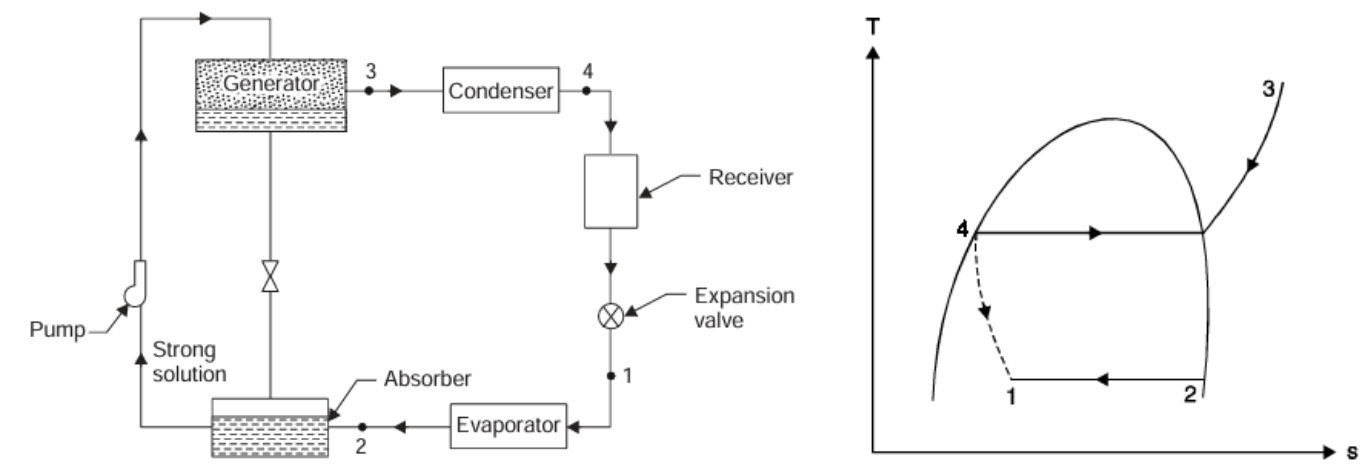
\includegraphics[width = 0.9\linewidth]{Figuras/U1/F1-CICLO_ABSORCION.png}
		\caption{Sistema simple de absorción de vapor.}\label{F1-Sistema simple de absorción de vapor.}
	\end{figure}

	En este sistema el trabajo realizado en la compresión es menor que en un ciclo de compresión de vapor, ya que el bombeo de un líquido requiere mucho menos trabajo que la compresión de vapor entre las mismas presiones, pero se requiere una entrada de calor hacia el generador, el calor se puede suministra mediante cualquier forma convincente, por ejemplo, calentamiento por vapor o gas.

	\subsubsection{Sistema práctico de absorción de vapor}

	\begin{figure}[H]
		\centering
		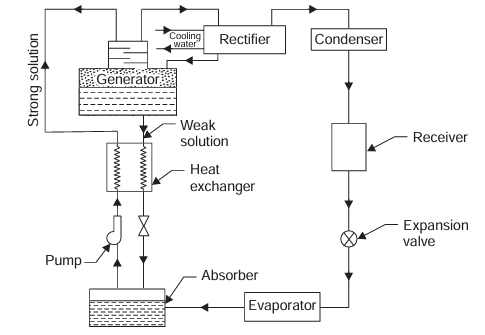
\includegraphics[width = 0.5\linewidth]{Figuras/U1/F1-CICLO_ABSORCION_PRACTICO.png}
		\caption{Sistema práctico de absorción de vapor.}\label{F1-Sistema práctico de absorción de vapor.}
	\end{figure}

	Consultando loa figura \ref{F1-Sistema práctico de absorción de vapor.} se llega a la conclusión que un sistema simple de absorció nde vapor puede proporcionar refrigeración, pero a una eficiencia baja. Por lo tanto, los accesorios siguientess se instalan para hacer el sistema más práctico y mejorar el desempeño y funcionamiento de lap lanta.

	\begin{enumerate}
		\item Cambiador de calor.
		
		Un cambiador de calor se ubica entre el generador y el absorbedsor. La solución concentrad,a que bombea del absorbedor al regeenrador, se debe calentar; y la solución diluida del generador al absorbedor se debe efnriar. Esto se efectúa por unintercambiador de calor y en consecuencia el costo del calentamiento del generador y el costo de enfriamiento del absorbedor es menor.

		\item Analizador.
		
		El analizado consiste en una serie de bandejas monjtadas arriba del generador. Su función principal es remover parcialmente parte de las partículas de agua no deseables asoociadas con el vapor de amoniaco que van hacia el condensador. Si estos vapores de aguas e permiten entrar al condensador pueden entrara a la válvula de expansión y congelarse; como resultado puede obstruir la tubería.

		\item Rectificador.
		
		Un rectificador es un cambiador de calor enfriado por agua que condensa el vapor de agua y algo de vapor de amoniaco y lo envía de regreso al generador. Así pues, la solución final o eliminación del porcentaje de vapor de agua tiene lugar en el rectificador.

	\end{enumerate}

	El coeficiente de desempeño de refrigeración está definido por 

	\begin{equation}
		COP = \dfrac{\text{Calor extraído del evaporador}}{\text{Calor sum. en el generador} + \text{Trabajo realizado por la bomba}}
	\end{equation}

	
	\section{Refrigerantes en instalaciones}
	\Biblio{\cite[pág. 772 a 780]{Rajput2011termodinamica} \cite[pág. 395 a 399]{DossatPDRefrigeracion}}

	

	Un refrigerante se define como cualquier sustancia que absorbe calor a través de su evaporación o condensación y lo pierde a través de su condensación en un sistema de refrigeración. El término refrigerante en el sentido más amplio también se aplica a medios de enfriamiento secundarios como las soluciones de agua fría o de salmuera. En general, los refrigerantes incluyen solo los medios de trabajo que pasan por el ciclo de evaporación, recuperación, compresión, condensación y licuefacción. Estas sustancias absorben calor en un lugar a un nivel bajo de la temperatura y lo rechazan en algún otro lugar ya con una temperatura y presión mayor. El rechazo de calor sucede a costa de cierto trabajo mecánico. Así pues, los medios fríos circulantes y los medios de enfriamiento no son refrigerantes primarios. EN los primeros días sólo se utilizaban cuatro refrigerantes: 

	\begin{itemize}
		\item Aire.
		\item Amoniaco ($NH_3$).
		\item Dióxido de carbono ($CO_2$).
		\item Dióxido de azufre ($SO_2$).
	\end{itemize}

	Estos poseían propiedades químicas, físicas y termodinámicas que permitían su aplicación y servicio eficiente en el diseño práctico de equipo de refrigeración. Todos los refrigerantes cambian de un estado líquido a un estado de vapor durante el proceso.

	\subsection{Clasificación de los refrigerantes}

	Los refrigerantes pueden clasificarse en refrigerantes primarios y refrigerantes secundarios.

	Los refrigerantes primarios son los medios de trabajo o portadores de calor que tienen una función de manera directa en el sistema de refrigeración y enfrían una sustancia mediante la absorción de calor latentes. Por ejemplo, amoniaco, dióxido de carbono, dióxido de azufre, cloruro de metlilo, cloruro de metileno, cloruro etílico, el grupo Freón, etc.

	Los refrigerantes secundarios son las sustancias circulando que primero se enfrían con ayuda de los refrigerantes primarios y luego se emplean para fines de enfriamiento. Por ejemplo, hielo, dióxido de carbono sólido, etc. Estos refrigerantes enfrían sustancias por medio de absorción de su calor sensible.

	Los refrigerantes primarios se agrupan de la siguiente manera:

	\begin{itemize}
		\item Compuestos de halocarburos. En este grupo se incluyen refrigerantes que contienen uno o más de tres alógenos, cloro y bromuro y se venden en el mercado con nombres de Freón, Genotrón, Isotrón y Aretón. Como los refrigerantes que pertenecen a este grupo tienen ventajas extraordinarias sobre los refrigerantes de otros grupos, tienen un campo de aplicación muy amplio para fines domésticos, comerciales e industriales.
		\item Azeótropos. Los refrigerantes azeótropos consisten de mezclas de sustancias diferentes. Estas sustancias no se pueden separar en sus componentes mediante destilación. Poseen propiedades termodinámicas fijas y no experimentan separación con cambios de temperaturas o presión. Se comportan como sustancias simples.
		\item Hidrocarburos. La mayoría de los refrigerantes de este grupo son compuestos orgánicos. Varios hidrocarburos se emplean con éxito en instalaciones comerciales e industriales. Casi todos estos poseen propiedades termodinámicas satisfactorias, pero son altamente inflamables.
		\item Compuestos inorgánicos. Antes de la introducción del grupo de hidrocarburos, estos refrigerantes fueron los de uso común para todos los fines.
		\item Compuestos orgánicos insaturados. Los refrigerantes que pertenecen a este grupo contienen etileno o propileno.
	\end{itemize}

	\subsubsection{Mezclas previsibles}

	Cuando se producen mezclas de refrigerantes y aceites, no debe haber ninguna reacción química entre un refrigerante y el aceite de lubricación del compresor. La miscibilidad del aceite es muy importante y que cierta cantidad de aceite se debe sacar del cárter del compresor con el vapor refrigerante caliente para lubricar de manera adecuada los émbolos y las válvulas de descarga.

	Cuando se presenta una mezcla entre el refrigerante y materiales constructivos, se debe contemplar la selección del material para contener el refrigerante. Los refrigerantes atacan algunos metales, por ejemplo, el amoniaco reacciona con el cobre, latón u otras aleaciones cuprosas en presencia de agua, por lo tanto, en sistemas con amoniaco los metales comunes utilizados son el hierro y el acero. El grupo freon no reacciona con el acero, cobre latón, zinc, estaño y aluminio, pero es corrosivo con el magnesio y el aluminio con 2\% de magnesio. Los refrigerantes del grupo freón tienden a disolver caucho natural en los empaques y sellos, pero el caucho sintético con neopreno es completamente adecuado. Los hidrocarburos hidrogenados pueden reaccionar con el zinc, pero no con el cobre, aluminio, hierro y acero.

	\subsubsection{Propiedades y usos de refrigerantes comunes}

	\begin{itemize}
		\item Aire.
		
		El aire no tiene costo, se presente con gran disponibilidad, es completamente seguro y no es tóxico. El COP de un ciclo de aire funcionando entre temperaturas de $80^\circ C$ y $-15^\circ C$ es un 30\% del valor ideal de Carnot.

		El aire fue uno de los primeros refrigerantes y se utilizó ampliamente en momentos donde se requirió un medio completamente no tóxico. Actualmente, debido a su bajo COP, se utiliza solo en zonas donde la eficiencia de funcionamiento es secundaria, como lo es la refrigeración aeronaval.

		\item Amoniaco ($NH_3$).

		El amoniaco es altamente tóxico e inflamable, pero tiene propiedades térmicas excelentes. Tiene el efecto refrigerante mayor por kilogramo de refrigerante, bajo desplazamiento volumétrico, es barato y bajo peso del líquido circulado por ton de refrigeración. Por todas estas razones tiene una alta eficiencia. Las presiones del evaporador y del condensador son $3.5bar$ y $13bar$ absolutas, respectivamente en condiciones de temperatura de $-15^\circ C$ Y $30^\circ C$.

		Se utiliza ampliamente en sistemas de compresión alternativa industrial y comercial donde una toxicidad alta es secundaria. Principalmente, su uso se da en plantas de hielo, plantas de empaque, almacenamientos fríos grandes y pistas de patinaje, entre otros. Se utiliza ampliamente como refrigerante en sistemas de absorción.
		
		Algunos detalles interesantes son que, el amoniaco nunca se debe emplear con cobre, latón y otras aleaciones de cobre. En lugar se debe utilizar hierro o acero en sistemas con amoniaco. Además, para la detección de fugas se utiliza una vela de azufre que emite un color blanco y denso cuando está presente un vapor de amoniaco.

		EL amoniaco es el único refrigerante fuera de los fluorocarburos que se usa bastante en la actualidad. Aunque es tóxico, algo inflamable y explosivo en ciertas condiciones, sus excelentes propiedades térmicas lo hacen ser un refrigerante ideal para fábricas de hielo, plantas empacadoras, pistas de patinaje, grandes almacenes de enfriamiento, etc. donde se cuenta con los servicios de personal experimentado  y donde su naturaleza tóxica es de poca consecuencia.

		El amoniaco es el refrigerante que tiene mas alto efecto refrigerante por libra, el cual, a pesar de su volumen específico alto en la condición de vapor, tiene una gran capacidad refrigerante con relativamente un desplazamiento pequeño del pistón.

		El punto de ebullición del amoniaco a la presión atmosférica estándar es de $-28^\circ F (-33^\circ C)$. Las presiones en el evaporador y el condensador a las condiciones de tonelada estándar de $5^\circ F (-15^\circ C)$ y  $86^\circ F (30^\circ C)$ son de $34.27lb/in^2 (2.37bar)$ y $169.2lb/in^2 (11.67bar)$. respectivamente, las cuales son moderadas, de tal manera que pueden usarse materiales de peso ligero en la construcción del equipo refrigerante. SIn embargo, la temperatura adiabática en la descarga es relativamente alta, siendo de $210^\circ F (99^\circ C)$ para las condiciones de toneladas estándar, por lo cual es adecuado tener enfriamiento con agua tanto en el cabezal como en el cilindro del compresor. DEbe también evitarse tener sobrecalentamiento alto en la succión para los sistemas de amoniaco.

		Aunque el anhidro de amoniaco puro no es corrosivo para todos los metales normalmente usados en los sistemas de refrigeración, en la presencia de humedad, el amoniaco se vuelve corrosivo para los metales no ferrosos,  tales como el cobre y el latón. Evidentemente que estos metales no deben emplearse en los sistemas de amoniaco.

		EL amoniaco no es miscible con el aceite y por lo mismo no se diluye en el aceite del cárter del cigüeñal del compresor. Sin embargo, deben hacerse los arreglos necesarios para eliminar el aceite del evaporador y deberá usarse un separador de aceite en el tubo de descarga de los sistemas de amoniaco.

		En los sistemas de amoniaco pueden usarse velas de azufre para detectar las fugas, con lo cual se produce un humo blanco denso enb la presencia del vapor de amoniaco, o también puede aplicarse una solución de jabón poniéndola alrededor de las juntas en la tubería, en cuyo caso la fuga se manifestaría mediante la aparición de burbujas.

		El amoniaco es fácil de conseguir y es el más barato de los refrigerantes comúnmente empleados. Estos dos hechos, junto con su estabilidad química, afinidad por el agua y no miscibilidad por el aceite, hacen al amoniaco ser un refrigerante ideal para ser usado en sistemas muy grandes donde la toxicidad no es un factor importante. Debido a su coeficiente de transferencia de calor relativamente alto y al consecuente mejoramiento de la razón de transferencia de calor, es el amoniaco particularmente adecuado para grandes instalaciones de enfriamiento de líquido. Al amoniaco se le usa con compresores reciprocantes tipo abierto, rotatorios y centrífugos. 

		\item Dióxido de azufre ($SO_2$).
		
		El dióxido de azufre es incoloro, extremadamente tóxico y tiene un olor acre irritante. Sin embargo, este no es explosivo ni irritante. Tiene una gravedad específica de 1.36. Funciona a bajas presiones y tiene un calor latente de vaporización bajo.

		En la actualidad se utiliza poco, sin embargo, se utilizaba en máquinas pequeñas en los primeros días de la refrigeración. 

		La fuga de dióxido de azufre se puede detectar acercando amoniaco acuoso a la fuga, esto emite un humo color blanco.

		\item Dióxido de carbono ($CO_2$).
		
		El dióxido de carbono es un gas incoloro e inoloro, y es más pesado que el aire, tiene una gravedad específica de $1.56$. No es tóxico, tampoco inflamable, explosivo ni corrosivo. Como desventaja, tiene presiones de funcionamiento extremadamente altas y un efecto refrigerante muy bajo.
		
		Este refrigerante ha recibido un suo limitado debido a los requerimientos de alta potencia por ton de refrigeración y las altas presiones de funcionamiento. En el pasado ha sido utilizado para refrigeración marina, para refrigeración en teatros, hoteles e instituciones debido a no ser tóxico. EN la actualidad su uso está limitado principalmente a la manufactura de hielo seco. 

		\item Cloruro de metilo ($CH_3 Cl$)

		El cloruro de metilo es incoloro con olor suave, dulce y no irritante. Tiene una gravedad específica líquida de 1 a presión atmosférica. No es inflamable ni tóxico.

		Se ha utilizado comúnmente en aplicaciones domésticas y comerciales. Nunca se debe emplear con aluminio.

		\item R11 (tricloro monofluoro metano).
		
		Se compone de un átomo de carbono, tres de cloruro y uno de flúor y no es corrosivo, tóxico ni inflamable. Debido a su composición disuelve caucho natural y tiene un punto de ebullición a $-24^\circ C$. Se mezcla completamente con el aceite mineral de lubricación en todas las condiciones. 

		Se utiliza para una capacidad de 50ton y mayor en pequeños edificios de oficinas y fábricas pequeñas. EN las plantas que emplean este refrigerante se utiliza un compresor centrífugo. 

		Para detectar sus fugas se utiliza un soplete de haluro.
		
		El R11 es un flurocarburo de la serie del metano que tiene punto de ebullición de valor $74.7^\circ F (23.7^\circ C)$ a presión atmosférica. Las presiones de funcionamiento a condiciones de tonelada estándar son $2.94lb/in^2 (0.2bar)$ y $18.19lb/in^2 $ $  (1.25bar)$. DEbido al pequeño valor de las presiones de funcionamiento y al desplazamiento del compresor relativamente alto, el R11 se emplea con compresores centrífugos, sobre todo en sistema de aire acondicionado para pequeñas oficinas en edificios, fábricas, tiendas de departamentos, teatros, etc. El R11 es ampliamente utilizado como refrigerante secundario y como solvente.

		Al igual que otros refrigerantes fluorocarburos, el R11 no es corrosivo ni tóxico y, no es inflamable, pero disuelve al hule natural. Para detectar sus fugas se usa una antorcha halida.

		\item R12 o freón 12.
		
		Este refrigerante no es tóxico, inflamable ni explosivo, por lo tanto es el refrigerante adecuado. Es completamente miscible con el aceite, por lo tanto simplifica el problema del retorno del aceite. Las presiones de funcionamiento del R12 en un evaporador y  condensador ante una ton estándar de refrigeración son 1.9 bar absoluta y 7.6 bar absoluta, respectivamente. SU calor latente a $-15^\circ C$ es $161.6kJ/kg$, el COP es $80\%$ del referente al ciclo Carnot. No se descompone incluso ante condiciones de funcionamiento extremas, se condensa a presión moderada y en condiciones atmosféricas.

		Su uso es adecuado para aplicaciones de alta, media y baja temperatura, se utiliza en aplicaciones domésticas. Es un aislante eléctrico excelente, por lo tanto se emplea en compresores de tipo hermético.

		Es probable que el refrigerante R12 en la actualidad sea el más ampliamente usado. Es un refrigerante seguro en el sentido que no es tóxico, no es inflamable y no es explosivo. Además, es un compuesto altamente estable que es muy difícil de que falle aun bajo condiciones extremas de operación. Sin embargo, al ponerlo en contacto con una flama abierta o con un elemento de calefacción eléctrica, el R12 se descompone en productos que son altamente tóxicos.

		Además de sus propiedades de seguridad, el hecho de que el R12 se condensa a una presión moderada bajo condiciones atmosféricas normales y que tenga una temperatura de ebullición de $-21.6^\circ F (-29.8^\circ C)$ a presión atmosférica, hace que este refrigerante sea muy apropiado para usarse en aplicaciones de alta, media y baja temperatura y con los tres tipos de compresores. EL R12 se le ha usado para enfriar salmuera a temperaturas bajas, como de $-110^\circ F (-80^\circ C)$ utilizando para ello compresores centrífugos de pasos múltiples.
		
		El hecho de que el R12 sea miscible en aceite bajo todas las condiciones de operación, no solo simplifica el problema del retorno del aceite, sino que también tiende a aumentar la eficiencia y la capacidad del sistema, en tanto que la acción solvente del refrigerante mantenga al evaporador y al condensador libres de partículas de aceite, que de otra manera tendería a reducir la capacidad  de transferencia de calor de esas dos unidades. 

		Aunque el efecto refrigerante por libra de R12 es relativamente pequeño en comparación con los demás refrigerantes populares, esto no es necesariamente una desventaja seria, de hecho, para los sistemas pequeños, el hecho de hacer circular un peso grande de R12 es una gran ventaja que permite llevar un control más preciso del líquido. En sistemas de gran capacidad, la desventaja del bajo valor de calor latente se ve compensada por la densidad alta que tiene en el evaporador, de tal manera que el desplazamiento del compresor requerido por tonelada de refrigeración no es mucho más grande que lo requerido por otros refrigerantes comunes. También la potencia requerida por tonelada de capacidad es comparablemente favorable con la requerida por los otros refrigerantes comunes.

		Se usa la antorcha de halida para detectar fugas.

		\item R13 o freón 13.
		
		El refrigerante R13 fue desarrollado para usarse en aplicaciones de temperatura ultra baja, generalmente en el paso inferior de dos o tres pasos de un sistema en cascada.

		La temperatura de ebullición del R13 es $-144.5^\circ F (-98^\circ C)$ a la presión atmosférica. La temperatura en el evaporador baja hasta $-150^\circ F (-100^\circ C)$ la temperatura crítica es $83.9^\circ F (28.9^\circ C)$. Al refrigerante R13 se le puede usar con los tres tipos de compresores debido a que su presión de condensación y desplazamiento del compresor son de valor moderado.

		El refrigerante R13 es un refrigerante seguro, no es miscible con el aceite, para detectar fugas se debe aplicar una antorcha halida.

		\item R22 o freón 22.
		
		El refrigerante R22 es superior al R12 en muchos aspectos. EL desplazamiento del compresor por ton de refrigeración es 60\% menor que el desplazamiento con R12. Además, el R22 es miscible con aceite a la temperatura del condensador, pero trata de separarse a temperatura del evaporador cuando el sistema se utiliza en aplicaciones de baja temperatura ($-90^\circ C$); en estos casos, se deben incorporar separadores de aceite para regresar el aceite del evaporador. Las presiones del evaporador y condensador a una ton estándar de refrigeración son mayores que las de R12. ($2.9bar$ y $11.9bar$). El R22 posee un bajo calor latente a $-15^\circ C$, el cual es $89kJ/kg$. La principal desventaja del R22 es su alta temperatura de descarga, que requiere enfriamiento por agua de la cabeza y del cilindro del compresor.

		El R22 se utiliza universalmente en sistemas de baja temperatura comerciales e industriales.

		El refrigerante R22 tiene un punto de ebullición a la presión atmosférica de \FC{-41.4}{-40.8}. Originalmente fue desarrollado como refrigerante para temperatura baja. Se le ha usado extensamente en congeladores domésticos y de granjas y en sistemas comerciales e industriales de baja temperatura, las temperaturas del evaporador son tan bajas como \FC{-125}{-87}. Actualmente se le usa sobre todo en acondicionadores de aire tipo paquete, por las limitaciones de espacio resulta una gran ventaja el valor relativamente pequeño del desplazamiento del compresor.

		Tanto las presiones de operación como la temperatura adiabática de la descarga son mayores para el R22 que para el R12. Los requerimientos de potencia son aproximadamente iguales.

		Debido a que la temperatura en la descarga del R22 es alta, la temperatura sobrecalentada en la succión debe conservarse en su valor mínimo, sobre todo cuando se usan unidades herméticas motor-compresor. En aplicaciones de temperatura baja, donde las relaciones de compresión son altas, se recomienda tener en enfriamiento con agua al cabezal y a los cilindros del compresor a fin de evitar sobrecalentamiento en el compresor. Los condensadores enfriados con aire empleados con el refrigerante R22, deben ser de tamaño generoso.

		Aunque el R22 es miscible con aceite en la sección de condensación a menudo suele separarse del aceite en el evaporador. La temperatura exacta a la cual ocurre la separación varía considerablemente con el tipo de aceite y con la cantidad de aceite mezclado con el refrigerante. Sin embargo, no se han tenido dificultades en el retorno del aceite después del evaporador cuando se tiene el diseño adecuado del serpentín del evaporador y de la tubería de succión. Se usan separadores de aceite cuando se utilizan evaporadores inundados y deberán tomarse medidas especiales para asegurarse del retorno del aceite desde el evaporador. Los separadores de aceite deberán usarse siempre en las aplicaciones de baja temperatura. 

		La principal desventaja del R22 sobre el R12 es que el R12 requiere un desplazamiento menor del compresor, siendo aproximadamente de 60\% del requerido para el R22. Por lo tanto, para un desplazamiento específico del compresor, la capacidad de refrigerante será aproximadamente 60\% mayor con R22 que con R12. Además, los tamaños de las tuberías por lo general son menores para el R22 que para el R12.

		La habilidad del refrigerante R22 para absorber la humedad es  considerablemente mayor que la del refrigerante R12 y, por lo tanto, se tienen menos problemas de congelamiento en los sistemas que usan R22.  Aunque algunos consideran que ello es una ventaja, esto es cuestionable por ser indeseable tener cualquier cantidad de humedad en el sistema refrigerante.

		Siendo un fluorocarburo, el R22 es un refrigerante seguro. Se puede usar antorcha de halida para detectar fugas.

		\item R113.
		
		El R113 a la presión atmosférica hierve a \FC{117.6}{47.5} las presiones de operación a condiciones de tonelada estándar son $0.9802 lb/in^2 $ $ (0.068bar)$ y $7.86 lb/in^2 $ $(0.208bar)$, respectivamente. Aunque el desplazamiento del compresor por ton es algo alto ($100.76ft^3/min \, ton$), la potencia requerida por tonelada se compara favorablemente con los demás refrigerantes comunes. Con este refrigerante se necesita usar compresor centrífugo por sus baja presiones de operación y por el desplazamiento grande requerido.

		Aunque principalmente se le usa en acondicionamiento de aire de confort también es empleado en procesos industriales de agua y salmuera hasta para \FC{0}{-18}.

		El R113 es un refrigerante seguro y se usa la antorcha halida para detectar fugas.

		\item R114.

		El R114, a presión atmosférica tiene su punto de ebullición de \FC{38.4}{3.6}. Las presiones de evaporación y condensación a condiciones de tonelada estándar son $6.75 lb/in^2 (0.89bar)$ y  $36.27 lb/in^2 (2.5bar)$ respectivamente. El desplazamiento requerido de compresor es relativamente bajo para una presión refrigerante baja ($19.59ft^3/min \, ton$) y  la potencia requerida se compara favorablemente con la de los otros refrigerantes comunes.
		
		Al R114 se le usa en compresores centrífugos en instalaciones muy grandes de acondicionamiento de aire comercial e industrial y para procesos industriales de enfriamiento de agua de hasta \FC{-70}{-57}. Se le usa con compresores rotatorios tipo aspa, en refrigeradores domésticos y en enfriadores pequeños de agua potable.

		Al igual que para el R22, el R114 es miscible en el aceite a las condiciones uqe se tienen en la sección de condensación, pero se separa del aceite en el evaporador. Sin embargo, debido al tipo de equipo usado con el R114 y las condiciones bajo las cuales se usa, el retorno de aceite no genera ningún tipo de problema.

		EL R114 es un refrigerante seguro. Se emplea la antorcha halida para detectar fugas.

		\item R500. 
		
		El R500 es una mezcla azeotrópica de refrigerante R12 (73.8\% en peso) y R152a (26.2\% en peso). A la presión atmosférica su punto de ebullición es \FC{-28}{-33}. Las presiones en el evaporador y condensador a condiciones estándar son  $16.4 lb/in^2 $ manométricas y  $113.4 lb/in^2$ manométricas, respectivamente. Aunque los requerimientos de potencia del R500 son aproximadamente iguales a los del R12 y R22, el desplazamiento requerido del compresor se encuentra entre medio del R22 y el R12.

		La principal ventaja del R500 está en el hecho de que su sustitución por el R12 presenta un aumento en la capacidad del compresor de aproximadamente 18\%. Esto hace posible usar el mismo compresor conectado directamente ya sea a 50 o 60hz de frecuencia con poco o ningún cambio en la capacidad de refrigerante o en los requerimientos de potencia.

		\item R502.
		
		El R502 es una mezcla azeotrópica de 42.8\% de R22 y 51.2\% de R115. Desarrollado originalmente como refrigerante de temperatura baja para reemplazar al R22 en algunas aplicaciones de temperatura baja y relación de compresión alta, el R502 ha sido ampliamente usado en un rango de temperaturas para almacenamiento congelado y frío y en algunas aplicaciones de aire acondicionado de confort, sobre todo donde se utilizan bombas de calor. La ventaja particular del R502 sobre el R22 es la temperatura adiabática baja que se tiene en la descarga, de \FC{99}{37.2}, comparada cn la de \FC{128}{53.3} a las condiciones de tonelada estándar. SIn embargo, tanto el desplazamiento del compresor como la capacidad por unidad de refrigerante son algo menores para el R502, así como las presiones de operación, aunque estas últimas permanecen en rangos moderados.
		
		El R502 a la presión barométrica estándar a una temperatura de ebullición de \FC{-49.8}{-45.4} y una temperatura crítica de \FC{179.9}{91.78}. No es inflamable y tampoco es tóxico y es baja su miscibilidad con el aceite. Se puede usar la antorcha halida para detectar fugas.

		\item R503.
		
		El refrigerante R503 es una mezcla azeotrópica de 40.1\% de R23 y 59.9 de R13. A la presión barométrica estándar tiene una temperatura de ebullición de \FC{-127.6}{88.7} y una temperatura crítica de \FC{67.1}{19.5}.

		El R503 es un refrigerante relativamente nuevo que puede reemplazar al R13 en el rango de temperatura de \FC{-100}{-73} hasta \FC{-150}{-101}. Con una temperatura en el evaporador de \FC{-120}{-84.4} y una temperatura de condensación de \FC{20}{6.67}, el desplazamiento requerido de compresor para el R503 es aproximadamente el 64\% del requerido por el R13 para la misma capacidad de refrigerante. SIn embargo, la presión de condensación es mayor para el R503, que para el R13.

		El R503 se usa en compresores reciprocantes en el paso inferior de un sistema de cascada, empleándose R12, R22 o R502 en el paso superior.

	\end{itemize}

	
	\section{Consideraciones de seguridad}
	\Biblio{\cite[pág. 29.6 a 29.10]{ashrae2017fundamentals} \cite[pág. 365 a 395, primera parte]{DossatPDRefrigeracion}}

	

	La national fire underwriters ha efectuado pruebas de toxicidad con los refrigerantes más comúnmente empleados. Como resultado de ello los refrigerantes están clasificados en seis grupos de acuerdo a su grado de toxicidad, los grupos están dispuestos en orden descendiente. Aquellos que están en el grupo 1 son altamente tóxicos y son capaces de causar la muerte o daños muy serios en concentraciones relativamente pequeñas y/o en periodos muy cortos de exposición. Por otra parte, aquellos que están clasificados en el grupo 6 son muy poco tóxicos, siendo capaces de causar efectos nocivos solo en concentraciones muy grandes. Debido a que el daño causado por el último grupo es más bien debido a deficiencias de oxígeno que a efectos nocivos del fluido, para todos los fines prácticos se considera que los fluidos del grupo 6 no son tóxicos. Sin embargo, como ya se ha indicado de algunos refrigerantes, aunque no sean tóxicos cuando se mezclan con el aire en su estado normal, están sujetos a descomposición cuando están en contacto con una flama o con un elemento eléctrico de calentamiento. Los productos de descomposición así formados, son altamente tóxicos y capaces de causar efectos nocivos en pequeñas concentraciones y en corta exposición. Esto es cierto 
	para todos los refrigerantes fluorocarburos.

	\subsection{Inflamabilidad y explosividad}

	Por otra parte, la serie de los hidrocarburos son altamente inflamables y explosivo, y deben usarse como refrigerantes para algunas aplicaciones especiales bajo la vigilancia de personal experimentados. Debido a sus excelentes propiedades térmicas de la serie de hidrocarburos, frecuentemente se utilizan en aplicaciones de temperatura muy bajas. En dichas instalaciones, el peligro en que se incurre se hace mínimo por el hecho de que el equipo está constantemente atendido por personal con experiencia en el uso y manejo de materiales explosivos.

	La ASSCMR\footnote{American Standar Safety Code for Mechanical Refrigeration.} da detalles de las condiciones y circunstancias bajo las cuales pueden ser usados con seguridad varios de los refrigerantes. Muchos de los códigos locales y ordenanzas que regulan el equipo de refrigeración están basadas en este código, el cual está mancomunadamente patrocinado por la ASHRAE y la ASA.
	
	El grado de peligro en que se incurre con el uso de refrigerantes tóxicos depende de varios factores, tales como la cantidad de refrigerante en relación con el tamaño del espacio dentro del cual se pueden tener fugas de refrigerante, el tipo de ocupación, de si se tengan flamas o fuego y de si el personal experimentado tenga la obligación de atender el equipo. Por ejemplo, si se tiene una cantidad muy pequeña de refrigerante altamente tóxico, representará poco peligro si se le usa en espacios relativamente grandes en donde es posible que en el caso de tener fugas, la concentración no llegue a un nivel de peligro. Además, el peligro inherente en el uso de refrigerantes tóxicos algunas veces es mitigado por el hecho de que los refrigerantes tóxicos despiden olores muy peculiares que tienden a dar aviso de su presencia. Entonces, los refrigerantes tóxicos generalmente son peligrosos para el caso de niños o de personas que por razones de enfermedad o confinamiento son incapaces de escapar de los humos. Actualmente, el amoniaco es el único refrigerante tóxico el cual es muy usado limitándose su uso a plantas paquete, fábricas de hielo y en almacenes de frío muy grandes los cuales son manejados por personal experimentado. \\ xx \\

	Según lo definido por la ASHRAE en el Standard 34, los refrigerantes pueden ser clasificados de acuerdo al peligro que puede generar su uso. La clasificación de la inflamabilidad y la toxicidad se presenta en seis grupos: A1, A2, A3, B1, B2 y B3. Los refrigerantes del grupo A1 son los menos peligrosos, mientras que los del grupo B3 son los más peligrosos.

	Con respecto a las clases A y B, estas representan el límite de exposición ocupacional que poseen; los refrigerantes de clase A poseen un límite de exposición ocupacional de 400ppm o mayor, mientras que los de clase B poseen un límite de exposición ocupacional menor a 400ppm.

	Pro otro lado, con respecto a la numeración:

	\begin{itemize}
		\item Clase 1: no generan propagación de flama en el aire a $60^\circ C$ y $101.3kPa$.
		\item Clase 2: exhiben propagación de flama en el aire a $60^\circ C$ y $101.3kPa$, donde su límite de ignición es mayor que $0.10kg/m^3$ a $23^\circ C$ y $101.3kPa$, y el calor de combustión es menor que $19000kJ/kg$.
		\item Variante clase 2L: son aquellos refrigerantes clase 2 que presentan una velocidad máxima de quemado no mayor a $100mm/s$ a $23^\circ C$ y $101.3kPa$.
		\item Clase 3: exhiben propagación de flama en el aire a $60^\circ C$ y $101.3kPa$, donde su límite de ignición es menor o igual que $0.10kg/m^3$ a $23^\circ C$ y $101.3kPa$, o el calor de combustión es mayor que $19000kJ/kg$.
	\end{itemize}

	Con respecto a la mezcla de refrigerantes, se debe tomar la clasificación de seguridad de aquel refrigerante que posea la peor clasificación. 

	\section{Refrigerantes secundarios}
	\Biblio{}

	\section{Conducción de fluidos refrigerantes}
	\Biblio{\cite[pág. 29.10 a 29.11]{ashrae2017fundamentals}}

	\subsection{Metales}

	Los refrigerantes halógenos pueden ser usados satisfactoriamente bajo condiciones normales con los metales más comunes, así como acero, hierro de fundición, cobre, bronce, estaño, plomo y aluminio. Bajo las condiciones más severas, muchos de los metales están sometidos a hidrólisis y descomposición térmica. El orden de los metales a presentar descomposición térmica frente a compuestos halogenados tiene el siguiente orden:

	\begin{equation}\nonumber
		\text{Aleaciones austeníticas Ni-Cr} < \text{18-8 Acero inoxidable} < \text{Niquel} < \text{Cobre}
	\end{equation}

		\begin{equation}\nonumber
		\text{Cobre} < \text{Acero 1040} < \text{Aluminio} < \text{Bronce} < \text{Cobre} < \text{Zinc} < \text{Plata}
	\end{equation}
	
	Este orden es aproximado, y existen algunas excepciones para algunos compuestos especiales. Las aleaciones de magnesio y aquellas de aluminio con más de 2\% de magnesio no son recomendadas para el uso con refrigerantes halógenos donde exista al menos un rastro de presencia de agua. EL zinc no es recomendado con CFC 113. Elementos de zinc y otros compuestos aleados con fluor deben ser usados de forma limitada, aunque no se ha observado ninguna situación fuera de lo normal en ambientes secos.
	Compuestos de aluminio, zinc o magnesio no deben ser nunca utilizados en contacto con cloruro de metilo. El amoniaco no debe ser utilizado con cobre, bronce u otra aleación que contenga cobre. 

	\subsection{Elastómeros}

	La hinchazón lineal de algunos elastómeros frente a la presencia del líquido de refrigerantes compuestos por HCFC y HFC es un factor a tener en cuenta. Estos factores, junto con el grado de dureza, la resistencia a la tracción y el grado de extracción, permiten definir la selección correcta del elastómero. Cuando existen otros fluidos junto al refrigerante, por ejemplo lubricantes, la combinación de estos y la acción que tengan sobre el elastómero debe ser considerada. 

	Otro inconveniente presente en los elastómeros es la permeabilidad frente a los fluidos. Ya que, en caso de no ser realmente permeables puede existir una fuba del propio refrigerante o presentarse un ingreso de humedad al propio sistema de refrigeración. La construcción de mangueras multicapas es utilizada significativamente para reducir el ingreso de agua y la pérdida de refrigerante. Una construcción típica de una manguera podría consistir en una cubierta exterior de elastómero de clorobutilo para reducir la entrada de agua, una capa de poliamida para reducir el refrigerante filtrado y un tubo interior de cloropreno. 

	\subsection{Plásticos}

	EL efecto del refrigerante a un material plástico debe ser analizado estrictamente bajo las condiciones de uso previsto, incluyendo la presencia de lubricantes. Los plásticos son generalmente mezclas de dos o más elementos, por lo que es difícil de predecir el efecto del refrigerante sobre el plástico. La masa y los cambios visuales frente al refrigerante pueden ser utilizados como referencia, pero los cambios en las propiedades internas del plástico deben ser examinadas. Los refrigerantes y lubricantes tuvieron poco efecto sobre la mayoría de los plásticos, aunque el acrilonitrilo-butadieno-estireno, el óxido de polifenileno y el policarbonato se vieron afectados lo suficiente como para ser considerados incompatibles.

	Se evaluó la compatibilidad de los refrigerantes R-134a y R-1234yf con los plásticos típicos utilizados en los sistemas de aire acondicionado automotriz. Cinco plásticos (poliéster, nailon, epoxi, tereftalato de polietileno y poliamida) se pusieron en contacto en tubos sellados que contenían los refrigerantes y el lubricante PAG, y se mantuvieron a 100 °C durante dos semanas. Veinticuatro horas después de finalizar la prueba, se evaluaron los cambios de masa y apariencia de los plásticos, obteniéndose esencialmente las mismas calificaciones positivas de ambos refrigerantes con los plásticos.

\newpage
\pagestyle{empty}